\chapter{二次规划与锥规划}
\label{chap:quadratic-conic-programming}

设三次观测告诉我们$x_1+x_2\approx4$、$x_1\approx1$、$x_2\approx0$，而$x_1,x_2$又必须非负、总和不超过$2$。这是带预算的最小二乘。换一个场合：要在两个圆盘的公共部分里找位置最低的点。再换一个：知道三个量两两之间的部分相关系数，要判断剩下的那个相关系数能取哪些值。

三件事看上去毫无关系，求解前却要回答同一个问题：目标和约束究竟是什么形状，能不能写成已有方法可以直接处理的形式？第一件事的目标是二次函数、约束是线性的；第二件事的约束是欧氏距离的上限；第三件事的约束是“某个对称矩阵的特征值非负”。这三种形状分别对应二次规划、二阶锥规划和半正定规划。

第~\ref{sec:cone-qp}节研究二次规划，看曲率和可行集怎样决定凸性、唯一性和计算方式。第~\ref{sec:cone-conic}节把线性规划的非负约束换成一般的闭凸锥，得到一种统一的模型和统一的对偶下界。

问题本身未必长成标准形式。第~\ref{sec:cone-rewrite}节研究怎样引入辅助变量而不改变问题，第~\ref{sec:cone-relax}节处理改不成凸问题的情形：放宽可行集，换来一个可以计算的下界。这两种操作的差别贯穿后半章，算出来的东西和原问题的关系也要分别核对。第~\ref{sec:cone-methods}节在同一个问题上比较各种写法的规模与代价。

\section{二次规划}
\label{sec:cone-qp}

拿到一个二次目标、线性约束的问题，于是要问：怎样在动手求解之前，判断它是否凸、解是否唯一、哪些线性代数运算可以直接拿来用？

\paragraph{从带预算的最小二乘开始}
回到章首的三次观测。把三条近似关系写成$\bm{D}\bm{x}\approx\bm{r}$，其中
\[
 \bm{D}=\begin{bmatrix}1&1\\1&0\\0&1\end{bmatrix},\qquad
 \bm{r}=\begin{bmatrix}4\\1\\0\end{bmatrix}.
\]
最小二乘的目标是$\frac12\lVert\bm{D}\bm{x}-\bm{r}\rVert_2^2$，约束是$\bm{x}\geq\bm{0}$和预算$x_1+x_2\leq2$。把这三条约束收集起来，就得到本节贯穿使用的问题。

展开平方，目标等于
\[
 \frac12\bm{x}^\top\bm{D}^\top\bm{D}\bm{x}-\bm{r}^\top\bm{D}\bm{x}+\frac12\lVert\bm{r}\rVert_2^2.
\]
常数项不影响最优解。记$\bm{Q}=\bm{D}^\top\bm{D}$、$\bm{q}=-\bm{D}^\top\bm{r}$，代入数据得到
\begin{equation}
 \bm{Q}=\begin{bmatrix}2&1\\1&2\end{bmatrix},\qquad
 \bm{q}=\begin{bmatrix}-5\\-4\end{bmatrix},\qquad
 \frac12\lVert\bm{r}\rVert_2^2=\frac{17}{2}.
 \label{eq:cone-running-data}
\end{equation}
于是目标是一个对称二次型加一个线性项，约束全是仿射的。

把这种形状抽象出来，就是下面的定义。为了不和最小二乘的$\bm{D},\bm{r}$混淆，约束的系数用另外的字母。

\begin{definition}[二次规划]
\label{def:cone-qp}
设$\bm{Q}\in\mathbb{R}^{n\times n}$对称，$\bm{q}\in\mathbb{R}^n$，$\bm{A}\in\mathbb{R}^{p\times n}$，$\bm{b}\in\mathbb{R}^p$，$\bm{G}\in\mathbb{R}^{m\times n}$，$\bm{h}\in\mathbb{R}^m$。问题
\begin{equation}
 \begin{aligned}
 \min_{\bm{x}\in\mathbb{R}^n}\quad&f(\bm{x})=\frac12\bm{x}^\top\bm{Q}\bm{x}+\bm{q}^\top\bm{x}\\
 \text{s.t.}\quad&\bm{A}\bm{x}=\bm{b},\quad\bm{G}\bm{x}\leq\bm{h}
 \end{aligned}
 \label{eq:cone-qp}
\end{equation}
称为\term{二次规划}（quadratic program，QP）。不等式逐分量理解。可行集$\bm{C}$是有限个闭半空间与超平面的交，即多面体。
\end{definition}

例中$p=0$，三条不等式对应
\[
 \bm{G}=\begin{bmatrix}1&1\\-1&0\\0&-1\end{bmatrix},\qquad
 \bm{h}=\begin{bmatrix}2\\0\\0\end{bmatrix}.
\]
若把预算换成每个分量各自的上下限$\bm{l}\leq\bm{x}\leq\bm{u}$，得到的是盒约束最小二乘，只是$\bm{G},\bm{h}$的内容不同，目标部分完全一样。

\paragraph{拿到二次规划先问三件事}
同一个形式~\eqref{eq:cone-qp}覆盖了难度相差极大的问题，差别由下面三件事决定。

\begin{enumerate}
 \item 曲率：$\bm{Q}$沿可以移动的方向是正、是零还是负？这决定问题是否凸、解是否唯一。
 \item 可行集：有哪些等式和不等式，集合是否有界？这决定解会不会落在边界上、会不会跑到无穷远。
 \item 线性代数结构：$\bm{Q}$和约束矩阵是否稀疏、是否已有分解？这决定一次计算要花多少。
\end{enumerate}

图~\ref{fig:cone-qp-budget}画出例子。蓝色椭圆是目标的等高线，中心$(2,1)$是不考虑约束时的最小二乘解。它的两个分量之和是$3$，超出预算，所以留在三角形内的最好位置落在预算边上。在解$\bm{x}^\star$处，负梯度仍然指向更低的椭圆中心，但沿这个方向走会离开可行集。

\begin{BookInlineFigure}
  \centering
  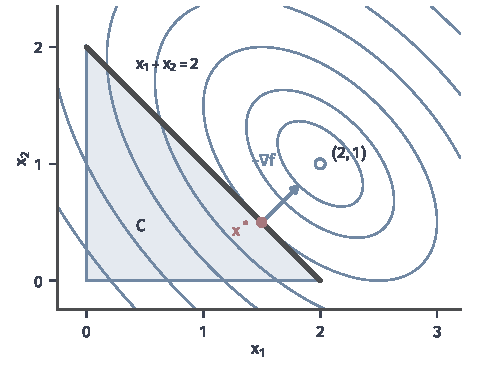
\includegraphics[width=84mm]{figures/05-optimization/06-constrained-optimization/matplotlib/cone-qp-budget/figure.pdf}
  \caption{带预算的最小二乘问题。蓝色椭圆是目标$\frac12\lVert\bm{D}\bm{x}-\bm{r}\rVert_2^2$的等高线，空心点$(2,1)$是无约束解。浅蓝三角形是可行集，深灰粗线是活动的预算约束，红点是解$\bm{x}^\star=(3/2,1/2)$。蓝色箭头是按比例缩短的负梯度，它垂直于预算边。}
  \label{fig:cone-qp-budget}
\end{BookInlineFigure}

\subsection{凸二次规划}
\label{sec:cone-convex-qp}

这一小节回答前两件事：目标在可行集上什么时候是一只碗，这只碗什么时候只有一个最低点。答案全部来自二次函数的一个恒等式。

\paragraph{一个恒等式}
二次函数的特别之处在于，它的高阶余项是零，局部信息就是全局信息。下面的引理把这句话写成精确的等式。

\begin{lemma}[二次函数的两个恒等式]
\label{lem:cone-quadratic-identities}
设$f$是式~\eqref{eq:cone-qp}中的二次函数，$\bm{Q}$对称。则$\nabla f(\bm{x})=\bm{Q}\bm{x}+\bm{q}$，且对任意$\bm{x},\bm{y}\in\mathbb{R}^n$和$\theta\in[0,1]$，
\begin{equation}
 f(\bm{y})=f(\bm{x})+\nabla f(\bm{x})^\top(\bm{y}-\bm{x})+\frac12(\bm{y}-\bm{x})^\top\bm{Q}(\bm{y}-\bm{x}),
 \label{eq:cone-exact-taylor}
\end{equation}
\begin{equation}
 \begin{aligned}
 f(\theta\bm{x}+(1-\theta)\bm{y})={}&\theta f(\bm{x})+(1-\theta)f(\bm{y})\\
 &-\frac12\theta(1-\theta)(\bm{x}-\bm{y})^\top\bm{Q}(\bm{x}-\bm{y}).
 \end{aligned}
 \label{eq:cone-chord-identity}
\end{equation}
\end{lemma}

\begin{proof}
记$\bm{d}=\bm{y}-\bm{x}$。直接展开，
\[
 f(\bm{x}+\bm{d})=\frac12\bm{x}^\top\bm{Q}\bm{x}+\bm{x}^\top\bm{Q}\bm{d}+\frac12\bm{d}^\top\bm{Q}\bm{d}+\bm{q}^\top\bm{x}+\bm{q}^\top\bm{d}.
\]
把含$\bm{d}$一次的两项合并成$(\bm{Q}\bm{x}+\bm{q})^\top\bm{d}$，就是式~\eqref{eq:cone-exact-taylor}。对$\bm{d}$的一次项系数就是梯度。

再证式~\eqref{eq:cone-chord-identity}。令$\bm{d}=\bm{x}-\bm{y}$，则$\theta\bm{x}+(1-\theta)\bm{y}=\bm{y}+\theta\bm{d}$。由式~\eqref{eq:cone-exact-taylor}，
\[
 f(\bm{y}+\theta\bm{d})=f(\bm{y})+\theta\nabla f(\bm{y})^\top\bm{d}+\frac12\theta^2\bm{d}^\top\bm{Q}\bm{d}.
\]
同一公式取步长$1$，得到
\[
 f(\bm{x})=f(\bm{y})+\nabla f(\bm{y})^\top\bm{d}+\frac12\bm{d}^\top\bm{Q}\bm{d}.
\]
于是
\[
 \theta f(\bm{x})+(1-\theta)f(\bm{y})=f(\bm{y})+\theta\nabla f(\bm{y})^\top\bm{d}+\frac12\theta\bm{d}^\top\bm{Q}\bm{d}.
\]
两式相减，差等于$\frac12(\theta^2-\theta)\bm{d}^\top\bm{Q}\bm{d}$，即式~\eqref{eq:cone-chord-identity}最后一项。
\end{proof}

式~\eqref{eq:cone-chord-identity}说，弦上的点比弦下面的函数值高出多少，完全由$(\bm{x}-\bm{y})^\top\bm{Q}(\bm{x}-\bm{y})$决定。线性项在其中不起作用。这一项为正，函数在这条线段上向下弯成碗；为负，则向上拱起。

因此要判断凸性，只需要看$\bm{Q}$在所有“两个可行点之差”上的符号。方向若永远走不到，它的曲率再负也无妨。

\paragraph{只看可行差方向}
把可行差张成的子空间记为
\begin{equation}
 \bm{V}=\operatorname{span}\{\bm{x}-\bm{y}:\bm{x},\bm{y}\in\bm{C}\},
 \label{eq:cone-feasible-subspace}
\end{equation}
并取$\bm{Z}$为一个矩阵，其各列构成$\bm{V}$的基。若$\bm{C}$中存在严格满足全部不等式的点，且$\bm{A}$的约束相容，则$\bm{V}=\ker\bm{A}$；此时$\bm{Z}$就是$\bm{A}$的零空间基。矩阵$\bm{Z}^\top\bm{Q}\bm{Z}$记录了$\bm{Q}$在可行方向上的全部曲率。

\begin{theorem}[可行集上的凸性]
\label{thm:cone-feasible-convexity}
设$\bm{C}$是式~\eqref{eq:cone-qp}的非空可行集，$\bm{Z}$的各列是$\bm{V}$的基。则
\begin{enumerate}
 \item $f$在$\bm{C}$上凸，当且仅当$\bm{Z}^\top\bm{Q}\bm{Z}\succeq\bm{0}$；
 \item $f$在$\bm{C}$上严格凸，当且仅当$\bm{Z}^\top\bm{Q}\bm{Z}\succ\bm{0}$。
\end{enumerate}
特别地，$\bm{Q}\succeq\bm{0}$时$f$在任何凸集上都凸。
\end{theorem}

\begin{proof}
先说明可行差足以探测$\bm{V}$中的每个方向。非空凸集在它的仿射包内有内点，取这样一个点$\bar{\bm{x}}$。存在$\varepsilon>0$，使得对$\bm{V}$中满足$\lVert\bm{d}\rVert_2\leq\varepsilon$的$\bm{d}$，都有$\bar{\bm{x}}+\bm{d}\in\bm{C}$。所以这样的$\bm{d}$是可行差，$\bm{V}$中任一非零方向乘上适当的正数后都是可行差。

设$f$在$\bm{C}$上凸。对$\bm{x}=\bar{\bm{x}}+\bm{d}$和$\bm{y}=\bar{\bm{x}}$，式~\eqref{eq:cone-chord-identity}中的最后一项必须不为正，故$\bm{d}^\top\bm{Q}\bm{d}\geq0$。缩放后对$\bm{V}$中全部方向成立，这就是$\bm{Z}^\top\bm{Q}\bm{Z}\succeq\bm{0}$。

反过来，若$\bm{Z}^\top\bm{Q}\bm{Z}\succeq\bm{0}$，则对任意$\bm{x},\bm{y}\in\bm{C}$，$\bm{x}-\bm{y}\in\bm{V}$，式~\eqref{eq:cone-chord-identity}中的最后一项不为正，$f$在$\bm{C}$上凸。

严格凸的情形相同。取$\bm{x}\neq\bm{y}$和$\theta\in(0,1)$，式~\eqref{eq:cone-chord-identity}说明弦严格高于函数，当且仅当$(\bm{x}-\bm{y})^\top\bm{Q}(\bm{x}-\bm{y})>0$。把上面两段的非负换成严格为正，论证逐句成立。
\end{proof}

最小二乘天然满足定理的条件。对$\bm{Q}=\bm{D}^\top\bm{D}$，有
\[
 \bm{d}^\top\bm{Q}\bm{d}=\lVert\bm{D}\bm{d}\rVert_2^2\geq0.
\]
所以带线性约束的最小二乘总是凸二次规划。严格凸与否取决于$\ker\bm{D}$与$\bm{V}$是否只交于零向量。例中$\bm{D}$列满秩，$\bm{Q}$的特征值是$1$和$3$，全空间正定。

\paragraph{连接线性方程与最优性条件}
没有约束时，最优条件是$\bm{Q}\bm{x}+\bm{q}=\bm{0}$，也就是最小二乘的正规方程$\bm{D}^\top\bm{D}\bm{x}=\bm{D}^\top\bm{r}$，其解法和选解可参考\BookChapterRef{chap:linear-solution-selection}{卷二第11章“线性方程与最小二乘的选解”}。例中由式~\eqref{eq:cone-running-data}解得无约束解$(2,1)$。

加上约束后，方程要换成第~\ref{chap:constrained-optimality}章的KKT条件。那一章证明了：约束全是仿射函数时，局部极小点满足KKT条件，不需要额外的约束规格。对问题~\eqref{eq:cone-qp}，KKT条件写成存在$\bm{\lambda}\in\mathbb{R}^m$和$\bm{\nu}\in\mathbb{R}^p$，使得
\begin{equation}
 \begin{gathered}
 \bm{Q}\bm{x}+\bm{q}+\bm{A}^\top\bm{\nu}+\bm{G}^\top\bm{\lambda}=\bm{0},\\
 \bm{A}\bm{x}=\bm{b},\qquad\bm{G}\bm{x}\leq\bm{h},\\
 \bm{\lambda}\geq\bm{0},\qquad\bm{\lambda}^\top(\bm{G}\bm{x}-\bm{h})=0.
 \end{gathered}
 \label{eq:cone-qp-kkt}
\end{equation}

凸性让这组条件从必要变成充分，也就成了全局最优的证书。

\begin{theorem}[凸二次规划的KKT证书]
\label{thm:cone-qp-kkt}
设$f$在$\bm{C}$上凸。可行点$\bm{x}$是问题~\eqref{eq:cone-qp}的全局最优解，当且仅当存在$\bm{\lambda},\bm{\nu}$使式~\eqref{eq:cone-qp-kkt}成立。
\end{theorem}

\begin{proof}
必要性是上面复述的结论，全局最优解当然是局部极小点。下面证充分性。任取可行点$\bm{y}$，记$\bm{d}=\bm{y}-\bm{x}$。由式~\eqref{eq:cone-exact-taylor}，
\[
 f(\bm{y})-f(\bm{x})=\nabla f(\bm{x})^\top\bm{d}+\frac12\bm{d}^\top\bm{Q}\bm{d}.
\]
$\bm{d}$是可行差，定理~\ref{thm:cone-feasible-convexity}给出$\bm{d}^\top\bm{Q}\bm{d}\geq0$。只需证第一项非负。

把驻定条件代入，并用$\bm{A}\bm{d}=\bm{0}$，得到
\[
 \nabla f(\bm{x})^\top\bm{d}=-\bm{\nu}^\top\bm{A}\bm{d}-\bm{\lambda}^\top\bm{G}\bm{d}=-\bm{\lambda}^\top\bm{G}\bm{d}.
\]
由互补条件$\bm{\lambda}^\top(\bm{G}\bm{x}-\bm{h})=0$，上式可以写成
\[
 -\bm{\lambda}^\top\bm{G}\bm{d}=-\bm{\lambda}^\top(\bm{G}\bm{y}-\bm{h})+\bm{\lambda}^\top(\bm{G}\bm{x}-\bm{h})=-\bm{\lambda}^\top(\bm{G}\bm{y}-\bm{h}).
\]
$\bm{\lambda}\geq\bm{0}$且$\bm{G}\bm{y}\leq\bm{h}$，所以右端非负。于是$f(\bm{y})\geq f(\bm{x})$。
\end{proof}

这个证书的好处是核对便宜。给出$\bm{x}$和$\bm{\lambda}$，只需做几次矩阵乘法，不必重新求解。

\begin{example}[核对预算问题的解]
\label{ex:cone-qp-kkt}
猜测预算活动、非负约束不活动。可行点$(3/2,1/2)$如何得来，下一小节再算，这里先核对。由式~\eqref{eq:cone-running-data}，
\[
 \nabla f(\bm{x})=\bm{Q}\bm{x}+\bm{q}=\begin{bmatrix}7/2\\5/2\end{bmatrix}+\begin{bmatrix}-5\\-4\end{bmatrix}=\begin{bmatrix}-3/2\\-3/2\end{bmatrix}.
\]
取$\bm{\lambda}=(3/2,0,0)$，则
\[
 \nabla f(\bm{x})+\bm{G}^\top\bm{\lambda}=\begin{bmatrix}-3/2\\-3/2\end{bmatrix}+\frac32\begin{bmatrix}1\\1\end{bmatrix}=\bm{0}.
\]
互补条件成立，因为预算的松弛量是$0$，另外两条约束的乘子是$0$。$\bm{\lambda}\geq\bm{0}$也成立。由定理~\ref{thm:cone-qp-kkt}，$(3/2,1/2)$是全局最优解。

最优值按$\frac12\lVert\bm{D}\bm{x}-\bm{r}\rVert_2^2$计算。残差是$\bm{D}\bm{x}-\bm{r}=(-2,1/2,1/2)$，于是
\[
 f^\star=\frac12\Bigl(4+\frac14+\frac14\Bigr)=\frac94.
\]
\end{example}

\paragraph{解的存在与唯一}
凸性不保证最优解存在。$\frac12x_1^2+x_2$的$\bm{Q}$半正定，在全平面上却无下界，沿$x_2\to-\infty$一路下降。有下界时情况好得多：二次函数只要在非空多面体上有下界，就一定取得最小值。这一结论称为Frank--Wolfe定理，它不要求凸性；证明要对约束个数作归纳，处理最小化序列沿回收方向发散的情形，篇幅较长，读者可查阅二次规划方面的专著。

这里有一点值得和一般光滑函数对比。第~\ref{chap:optimization}章的$e^x$在全直线上有下界$0$，却取不到。二次函数不会有这样的渐近行为。

唯一性由曲率直接给出，而且只需要看可行差方向。

\begin{theorem}[存在唯一性的充分条件]
\label{thm:cone-qp-unique}
设$\bm{C}$非空，且对$\bm{V}$中每个非零$\bm{d}$都有$\bm{d}^\top\bm{Q}\bm{d}>0$。则问题~\eqref{eq:cone-qp}恰有一个最优解。
\end{theorem}

\begin{proof}
先证存在。取$\bar{\bm{x}}\in\bm{C}$，$\bm{C}$中的点都可写成$\bar{\bm{x}}+\bm{Z}\bm{u}$。此时$f$成为$\bm{u}$的二次函数，其二次项矩阵$\bm{Z}^\top\bm{Q}\bm{Z}$正定，故$\lVert\bm{u}\rVert_2\to\infty$时函数值趋于$+\infty$，下水平集有界。可行集是闭集，所以下水平集紧，第~\ref{chap:optimization}章的存在定理给出最优解。

再证唯一。设$\bm{x}\neq\bm{y}$都是最优解，中点$\bm{z}=(\bm{x}+\bm{y})/2$可行。对式~\eqref{eq:cone-chord-identity}取$\theta=1/2$，并记$\bm{d}=\bm{x}-\bm{y}\in\bm{V}$，得到
\[
 f(\bm{z})=f^\star-\frac18\bm{d}^\top\bm{Q}\bm{d}<f^\star.
\]
这与$f^\star$是最优值矛盾。
\end{proof}

定理要求的是$\bm{V}$上正定，不是全空间正定。图~\ref{fig:cone-qp-uniqueness}比较了三种情形。

\begin{BookInlineFigure}
  \centering
  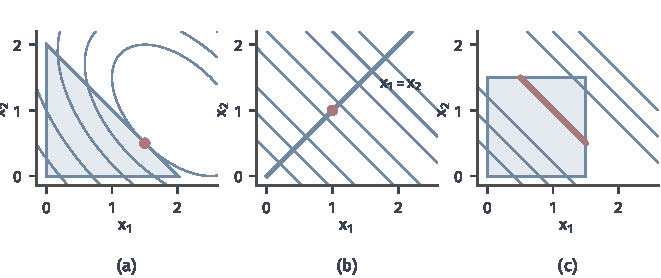
\includegraphics[width=112mm]{figures/05-optimization/06-constrained-optimization/matplotlib/cone-qp-uniqueness/figure.pdf}
  \caption{曲率与解的唯一性，蓝线是目标等高线，红色是解集。(a)预算问题，$\bm{Q}$全空间正定，解唯一。(b)目标$\frac12(x_1+x_2-2)^2$的$\bm{Q}$奇异，等高线是平行直线；约束直线$x_1=x_2$与谷底方向横截，解唯一。(c)同一目标，可行集是正方形$[0,3/2]^2$，平坦方向$(1,-1)$落在可行差内，解集是一条线段。}
  \label{fig:cone-qp-uniqueness}
\end{BookInlineFigure}

(b)中的目标来自只有一次观测的最小二乘，$\bm{D}=\begin{bmatrix}1&1\end{bmatrix}$，$\bm{r}=(2)$，于是$\bm{Q}=\begin{bmatrix}1&1\\1&1\end{bmatrix}$奇异，其零空间由$(1,-1)$张成。约束$x_1=x_2$使$\bm{V}$由$(1,1)$张成，而
\[
 (1,1)\,\bm{Q}\,(1,1)^\top=4>0.
\]
所以在可行直线上目标严格凸，解$(1,1)$唯一。全空间正定不是必要条件。

(c)中可行集仍是平面区域，平坦方向$(1,-1)$属于$\bm{V}$，定理的条件不成立，结论也确实不成立：线段$x_1+x_2=2$上的点全部最优，目标值都是$0$。

$\bm{V}$上正定同样不是唯一性的必要条件。考虑$\frac12x_1^2+x_2$，约束$x_2\geq0$。这里$\bm{V}=\mathbb{R}^2$，方向$(0,1)$的曲率为零，但线性项把解推到边界上：目标在可行集上非负，且只在原点为零，解唯一。线性规划是更极端的情形，$\bm{Q}=\bm{0}$，解却常常是唯一的顶点。

\paragraph{解集与可复用的运算}
凸二次规划的解不唯一时，解集也有规律。设$\bm{x},\bm{y}$都最优，式~\eqref{eq:cone-chord-identity}迫使$\bm{d}^\top\bm{Q}\bm{d}=0$，其中$\bm{d}=\bm{x}-\bm{y}$。$\bm{Q}\succeq\bm{0}$时这又推出$\bm{Q}\bm{d}=\bm{0}$，所以各最优解的梯度相同。解集上变的只有沿平坦方向的位置，不变的是梯度和最优值。

至于第三件事，二次规划的计算几乎都落到线性方程上。$\bm{Q}=\bm{D}^\top\bm{D}$时，$\bm{D}$的QR分解可以反复使用；求解过程换一组活动约束时，只需更新分解，不必重做。求解的形式与代价要到不等式的处理方法确定后才能比较，下一小节先看只有等式的情形。

\subsection{等式约束二次问题}
\label{sec:cone-equality-qp}

假如已经知道哪些不等式在解处活动，把它们当作等式，问题就只剩等式约束。这一小节研究
\begin{equation}
 \min_{\bm{x}}\ \frac12\bm{x}^\top\bm{Q}\bm{x}+\bm{q}^\top\bm{x}\quad\text{s.t.}\quad\bm{A}\bm{x}=\bm{b},
 \label{eq:cone-eqp}
\end{equation}
其中$\bm{A}\in\mathbb{R}^{p\times n}$行满秩，$p<n$。要回答的问题是：它能否化成一次线性方程，什么时候这个方程给出的确实是极小点？

例子取预算恰好用完的情形：$\bm{A}=\begin{bmatrix}1&1\end{bmatrix}$，$b=2$，$\bm{Q},\bm{q}$如式~\eqref{eq:cone-running-data}。可行集是平面上的一条直线。

可行集是一张平的“纸”，有两种自然的处理方式。一种是在纸上另取坐标，把问题变成无约束问题，只看纸面上的碗。另一种是留在原坐标里，引入乘子，把“不许离开纸面”变成方程。

\paragraph{零空间参数化}
取一个特解$\bm{x}_{\mathrm{p}}$满足$\bm{A}\bm{x}_{\mathrm{p}}=\bm{b}$，取$\bm{Z}\in\mathbb{R}^{n\times(n-p)}$，其各列是$\ker\bm{A}$的基。每个可行点都唯一地写成
\begin{equation}
 \bm{x}=\bm{x}_{\mathrm{p}}+\bm{Z}\bm{u},\qquad\bm{u}\in\mathbb{R}^{n-p}.
 \label{eq:cone-nullspace-param}
\end{equation}
约束被消去，$\bm{u}$可以取任意值。

把式~\eqref{eq:cone-nullspace-param}代入目标，并用式~\eqref{eq:cone-exact-taylor}以$\bm{x}_{\mathrm{p}}$为中心展开，得到$\bm{u}$的二次函数
\begin{equation}
 \varphi(\bm{u})=f(\bm{x}_{\mathrm{p}})+\bigl(\bm{Z}^\top(\bm{Q}\bm{x}_{\mathrm{p}}+\bm{q})\bigr)^\top\bm{u}+\frac12\bm{u}^\top\bm{Z}^\top\bm{Q}\bm{Z}\bm{u}.
 \label{eq:cone-reduced-objective}
\end{equation}
矩阵$\bm{Z}^\top\bm{Q}\bm{Z}$称为\term{约化Hessian}（reduced Hessian），它是目标在纸面上的曲率。令梯度为零，得到约化方程
\begin{equation}
 \bm{Z}^\top\bm{Q}\bm{Z}\,\bm{u}=-\bm{Z}^\top(\bm{Q}\bm{x}_{\mathrm{p}}+\bm{q}).
 \label{eq:cone-reduced-equation}
\end{equation}

在例子中取特解$\bm{x}_{\mathrm{p}}=(2,0)$和方向$\bm{z}=(1,-1)$。约化Hessian是一个数：
\[
 \bm{z}^\top\bm{Q}\bm{z}=2-1-1+2=2.
\]
$\bm{x}_{\mathrm{p}}$处的梯度是
\[
 \bm{Q}\bm{x}_{\mathrm{p}}+\bm{q}=\begin{bmatrix}4\\2\end{bmatrix}+\begin{bmatrix}-5\\-4\end{bmatrix}=\begin{bmatrix}-1\\-2\end{bmatrix}.
\]
它在$\bm{z}$上的投影是$\bm{z}^\top(\bm{Q}\bm{x}_{\mathrm{p}}+\bm{q})=1$。把两个数代入式~\eqref{eq:cone-reduced-equation}，得到
\[
 2u=-1,\qquad u^\star=-\frac12.
\]
于是
\[
 \bm{x}^\star=\begin{bmatrix}2\\0\end{bmatrix}-\frac12\begin{bmatrix}1\\-1\end{bmatrix}=\begin{bmatrix}3/2\\1/2\end{bmatrix}.
\]
这个点的两个分量都是正的，所以它也满足原来的非负约束，这正是例~\ref{ex:cone-qp-kkt}核对过的解。

图~\ref{fig:cone-qp-nullspace}(b)画出约化后的一元函数$\varphi(u)=u^2+u+5/2$。原问题的约束已经不见了，剩下的是一个普通的抛物线。

\begin{BookInlineFigure}
  \centering
  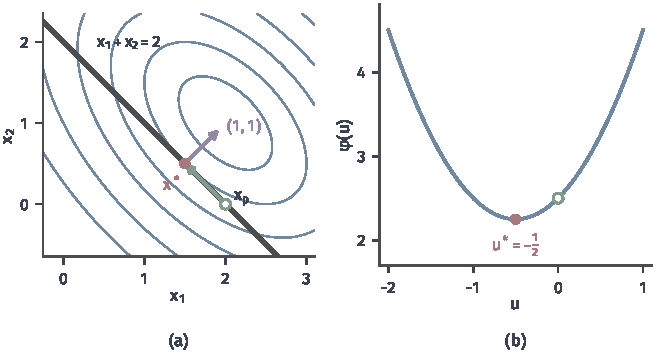
\includegraphics[width=112mm]{figures/05-optimization/06-constrained-optimization/matplotlib/cone-qp-nullspace/figure.pdf}
  \caption{预算恰好用完时的二次问题。(a)深灰粗线是可行直线，蓝线是目标等高线。从特解$\bm{x}_{\mathrm{p}}=(2,0)$（绿色空心点）沿零空间方向走到解（红点），绿色箭头是位移$u^\star\bm{z}$。紫色箭头是约束的法向$(1,1)$，解处的等高线与直线相切，梯度沿这个方向。(b)沿直线的一元函数$\varphi(u)=u^2+u+5/2$，空心点和红点对应(a)中的$\bm{x}_{\mathrm{p}}$与解。}
  \label{fig:cone-qp-nullspace}
\end{BookInlineFigure}

\paragraph{带乘子的块线性方程}
第二种做法不换坐标。对式~\eqref{eq:cone-eqp}写KKT条件，没有不等式，式~\eqref{eq:cone-qp-kkt}只剩两行，它们都是线性的。写成块形式：
\begin{equation}
 \begin{bmatrix}\bm{Q}&\bm{A}^\top\\\bm{A}&\bm{0}\end{bmatrix}
 \begin{bmatrix}\bm{x}\\\bm{\nu}\end{bmatrix}
 =\begin{bmatrix}-\bm{q}\\\bm{b}\end{bmatrix}.
 \label{eq:cone-kkt-system}
\end{equation}
左端的矩阵称为\term{KKT矩阵}（KKT matrix）。它对称，但不定，下方块是零。

例中方程组是
\[
 \begin{bmatrix}2&1&1\\1&2&1\\1&1&0\end{bmatrix}
 \begin{bmatrix}x_1\\x_2\\\nu\end{bmatrix}
 =\begin{bmatrix}5\\4\\2\end{bmatrix}.
\]
前两行相减消去$\nu$，得到$x_1-x_2=1$。第三行给出$x_1+x_2=2$。两式联立，
\[
 x_1=\frac32,\qquad x_2=\frac12.
\]
再代回第一行，
\[
 \nu=5-2x_1-x_2=\frac32.
\]
得到的$\bm{x}$与零空间参数化相同，还多了一个乘子。乘子的含义是预算的影子价格：预算增加一点点，最优值约按$\nu$的速率下降，这种变化率的一般讨论在第~\ref{chap:parametric-sensitivity}章。

两种做法解的是同一组条件。约束$\bm{A}\bm{x}=\bm{b}$由参数化自动满足，而$\ker\bm{A}$的正交补是$\bm{A}^\top$的列空间，所以下面两件事等价：
\begin{equation}
 \bm{Q}\bm{x}+\bm{q}\in\operatorname{range}(\bm{A}^\top)
 \quad\Longleftrightarrow\quad
 \bm{Z}^\top(\bm{Q}\bm{x}+\bm{q})=\bm{0}.
 \label{eq:cone-kkt-reduced-equivalence}
\end{equation}
左边是块方程第一行“存在$\bm{\nu}$”的说法，右边代入式~\eqref{eq:cone-nullspace-param}就是约化方程。

表~\ref{tab:cone-eqp-compare}比较两种做法的计算任务。

\begin{BookInlineTable}
  \centering
  \begin{tabular}{lll}
    \toprule
    & 零空间参数化 & 块线性方程\\
    \midrule
    需要准备 & 特解与零空间基$\bm{Z}$ & 无\\
    解的方程 & $(n-p)$阶，常可用Cholesky & $(n+p)$阶，对称不定\\
    适合的情形 & $n-p$小，$\bm{Z}$易得 & $\bm{Q}$、$\bm{A}$稀疏\\
    副产品 & 乘子需另算 & 直接得到乘子\\
    \bottomrule
  \end{tabular}
  \caption{等式约束二次问题的两种解法。$\bm{Z}$通常来自$\bm{A}^\top$的QR分解，$\bm{Q}$、$\bm{A}$稀疏时$\bm{Z}$和$\bm{Z}^\top\bm{Q}\bm{Z}$可能变稠密。}
  \label{tab:cone-eqp-compare}
\end{BookInlineTable}

\paragraph{唯一可解的条件}
块方程什么时候有唯一解？式~\eqref{eq:cone-kkt-reduced-equivalence}提示答案取决于约化Hessian，而不是$\bm{Q}$本身。

\begin{theorem}[KKT矩阵的可逆性]
\label{thm:cone-kkt-invertible}
设$\bm{A}\in\mathbb{R}^{p\times n}$行满秩，$\bm{Z}$的各列是$\ker\bm{A}$的基。则
\begin{enumerate}
 \item KKT矩阵可逆，当且仅当$\bm{Z}^\top\bm{Q}\bm{Z}$可逆；
 \item 若$\bm{Z}^\top\bm{Q}\bm{Z}\succ\bm{0}$，则式~\eqref{eq:cone-kkt-system}有唯一解，其中的$\bm{x}$是问题~\eqref{eq:cone-eqp}唯一的全局最优解。
\end{enumerate}
\end{theorem}

\begin{proof}
设$(\bm{d},\bm{w})$在KKT矩阵的零空间中，即
\[
 \bm{Q}\bm{d}+\bm{A}^\top\bm{w}=\bm{0},\qquad\bm{A}\bm{d}=\bm{0}.
\]
由第二式可写$\bm{d}=\bm{Z}\bm{u}$。第一式左乘$\bm{Z}^\top$，因为$\bm{A}\bm{Z}=\bm{0}$，得到$\bm{Z}^\top\bm{Q}\bm{Z}\bm{u}=\bm{0}$。

若$\bm{Z}^\top\bm{Q}\bm{Z}$可逆，则$\bm{u}=\bm{0}$，$\bm{d}=\bm{0}$。此时第一式成为$\bm{A}^\top\bm{w}=\bm{0}$，$\bm{A}$行满秩推出$\bm{w}=\bm{0}$。所以KKT矩阵可逆。

反过来，若存在$\bm{u}\neq\bm{0}$使$\bm{Z}^\top\bm{Q}\bm{Z}\bm{u}=\bm{0}$，令$\bm{d}=\bm{Z}\bm{u}\neq\bm{0}$。则$\bm{Q}\bm{d}$与$\ker\bm{A}$正交，属于$\operatorname{range}(\bm{A}^\top)$，存在$\bm{w}$使$\bm{Q}\bm{d}+\bm{A}^\top\bm{w}=\bm{0}$。$(\bm{d},\bm{w})$是非零的零空间向量，KKT矩阵奇异。第一条得证。

第二条的可逆性由第一条给出。此时$\varphi$严格凸，其唯一驻点是唯一的全局极小点；由式~\eqref{eq:cone-kkt-reduced-equivalence}，这个驻点正是块方程解中的$\bm{x}$。
\end{proof}

定理中的“行满秩”也是必需的。若$\bm{A}$行亏秩，存在$\bm{w}\neq\bm{0}$使$\bm{A}^\top\bm{w}=\bm{0}$，$(\bm{0},\bm{w})$就在零空间里，块方程要么无解，要么乘子不唯一。

\paragraph{可逆不等于极小}
线性方程组非奇异，只说明驻点存在且唯一，并不说明驻点是极小点。第一条与第二条之间差的正是约化曲率的符号。

取$\bm{Q}=\operatorname{diag}(1,-1)$，$\bm{q}=\bm{0}$，约束是过原点的直线，方向为$\bm{z}$。图~\ref{fig:cone-qp-reduced}比较了三个方向。目标沿直线$\bm{x}=s\bm{z}$的值是$\frac12s^2\bm{z}^\top\bm{Q}\bm{z}$，约化Hessian就是数$\bm{z}^\top\bm{Q}\bm{z}$。

\begin{BookInlineFigure}
  \centering
  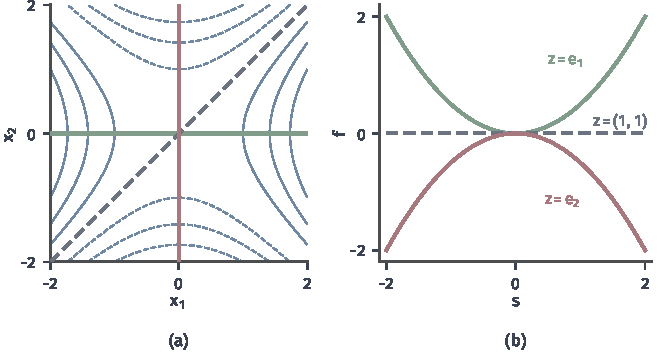
\includegraphics[width=112mm]{figures/05-optimization/06-constrained-optimization/matplotlib/cone-qp-reduced/figure.pdf}
  \caption{约化曲率决定驻点的性质。目标$\frac12(x_1^2-x_2^2)$，$\bm{q}=\bm{0}$。(a)蓝线是等高线（实线为正值，虚线为负值），三条直线是过原点的可行集。(b)目标沿每条直线的取值，横轴是直线上的坐标。绿线的约化曲率为$1$，灰色虚线为$0$，红线为$-1$。}
  \label{fig:cone-qp-reduced}
\end{BookInlineFigure}

表~\ref{tab:cone-reduced-cases}列出三种结果。

\begin{BookInlineTable}
  \centering
  \begin{tabular}{llll}
    \toprule
    方向$\bm{z}$ & $\bm{z}^\top\bm{Q}\bm{z}$ & KKT矩阵 & 原点的性质\\
    \midrule
    $(1,0)$ & $1$ & 可逆 & 唯一全局极小点\\
    $(1,1)$ & $0$ & 奇异 & 整条直线都是驻点\\
    $(0,1)$ & $-1$ & 可逆 & 沿直线的极大点，问题无下界\\
    \bottomrule
  \end{tabular}
  \caption{$\bm{Q}=\operatorname{diag}(1,-1)$、$\bm{q}=\bm{0}$时，约束直线的方向决定KKT矩阵和驻点的性质。}
  \label{tab:cone-reduced-cases}
\end{BookInlineTable}

第三行是要警惕的情形。此时约束是$x_1=0$，$\bm{A}=\begin{bmatrix}1&0\end{bmatrix}$，块方程的矩阵
\[
 \begin{bmatrix}1&0&1\\0&-1&0\\1&0&0\end{bmatrix}
\]
行列式为$1$，可逆，解是$\bm{x}=\bm{0}$、$\nu=0$。求解器不会报告任何异常，但$(0,s)$处的目标是$-\frac12s^2$，$\bm{x}=\bm{0}$是沿可行直线的最高点。

所以解完块方程还要核对约化曲率。不想构造$\bm{Z}$时可以看KKT矩阵的惯性：$\bm{A}$行满秩时，KKT矩阵恰有$n$个正特征值、$p$个负特征值，当且仅当$\bm{Z}^\top\bm{Q}\bm{Z}\succ\bm{0}$，而对称不定分解能直接读出惯性\scite{math-nocedal2006numerical}。

含不等式时，还要决定哪些不等式按等式处理，这个选择问题以及逐步调整的求解方法在第~\ref{chap:sequential-quadratic-programming}章展开。

\subsection{非凸二次问题}
\label{sec:cone-nonconvex-qp}

$\bm{Q}$在可行差方向上有负曲率时，前面的两个定理都不能用。这一小节要弄清：负曲率到底造成什么后果，约束又能挽回多少？

\paragraph{一个负曲率的例子}
考虑$\bm{Q}=\operatorname{diag}(1,-1)$的目标
\begin{equation}
 f(\bm{x})=\frac12x_1^2-\frac12x_2^2+\frac14x_2.
 \label{eq:cone-nonconvex-objective}
\end{equation}
沿$x_1$方向是碗，沿$x_2$方向是倒扣的碗。

先不加约束。唯一的驻点由$x_1=0$和$-x_2+\frac14=0$给出，是$\mathrm{S}=(0,1/4)$。沿$x_2$方向走，目标趋于$-\infty$，所以这个问题无下界，驻点是鞍点。

现在加上$-1\leq x_2\leq1$。约束切断了$x_2$方向的无限下降，$x_1$方向的目标又非负，所以目标在可行集上有下界。这就是图~\ref{fig:cone-qp-nonconvex}(a)中的带形区域。

\begin{BookInlineFigure}
  \centering
  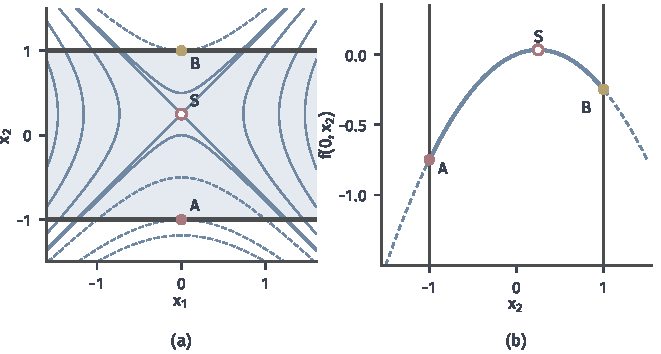
\includegraphics[width=112mm]{figures/05-optimization/06-constrained-optimization/matplotlib/cone-qp-nonconvex/figure.pdf}
  \caption{非凸二次问题的三个KKT点。目标$\frac12x_1^2-\frac12x_2^2+\frac14x_2$，可行集$-1\leq x_2\leq1$。(a)浅蓝带形是可行集，深灰粗线是约束边界，蓝线是等高线（虚线为负的较低水平）。红色实心点A是全局极小点，黄点B是局部极小点，红色空心点S是鞍点。(b)沿$x_1=0$的目标值，两条竖线之外不可行（虚线）。}
  \label{fig:cone-qp-nonconvex}
\end{BookInlineFigure}

\paragraph{KKT点的逐个判别}
约束写成$x_2-1\leq0$和$-x_2-1\leq0$，乘子分别记$\lambda_1,\lambda_2$。驻定条件给出$x_1=0$，以及
\[
 -x_2+\frac14+\lambda_1-\lambda_2=0.
\]
两条约束不能同时活动，所以按活动约束只有三种情形，每一种都是一个线性方程，结果列在表~\ref{tab:cone-nonconvex-kkt}中。

\begin{BookInlineTable}
  \centering
  \begin{tabular}{llll}
    \toprule
    点 & 活动约束 & 乘子 & 目标值\\
    \midrule
    $\mathrm{A}=(0,-1)$ & $x_2\geq-1$ & $\lambda_2=5/4$ & $-3/4$\\
    $\mathrm{B}=(0,1)$ & $x_2\leq1$ & $\lambda_1=3/4$ & $-1/4$\\
    $\mathrm{S}=(0,1/4)$ & 无 & $0$ & $1/32$\\
    \bottomrule
  \end{tabular}
  \caption{目标~\eqref{eq:cone-nonconvex-objective}在带形可行集上的三个KKT点。}
  \label{tab:cone-nonconvex-kkt}
\end{BookInlineTable}

三个点都满足一阶条件，性质却各不相同。判别要用第~\ref{chap:constrained-optimality}章的二阶条件：在乘子为正的活动约束的切方向上看曲率。

在A和B处，活动约束的乘子都为正，临界方向只有$(d_1,0)$，曲率$d_1^2>0$，所以二者都是严格局部极小点。在S处没有活动约束，$\bm{Q}$本身不定，沿$(0,1)$的曲率为负，所以S是鞍点。

比较目标值，A是全局极小点，B只是局部极小点。

\paragraph{不能继承的全局证书}
B满足全部KKT条件，却不是全局最优解。定理~\ref{thm:cone-qp-kkt}的证明在这里断在哪一步？取$\bm{x}=\mathrm{B}$、$\bm{y}=\mathrm{A}$，$\bm{d}=(0,-2)$。式~\eqref{eq:cone-exact-taylor}的两部分分别是
\[
 \nabla f(\mathrm{B})^\top\bm{d}=\Bigl(-\frac34\Bigr)(-2)=\frac32,\qquad
 \frac12\bm{d}^\top\bm{Q}\bm{d}=-2.
\]
一阶部分依然非负，这是KKT条件保证的。但二次部分为负，而且绝对值更大，两者之和是$-1/2$，恰好等于$f(\mathrm{A})-f(\mathrm{B})$。

表~\ref{tab:cone-nonconvex-feasible}把局部最优、鞍点和无下界并列起来。若只保留上界$x_2\leq1$、去掉下界，B依然是严格局部极小点，问题却变成无下界。局部信息看不出全局的命运。

\begin{BookInlineTable}
  \centering
  \begin{tabular}{lll}
    \toprule
    可行集 & 负曲率方向 & 结论\\
    \midrule
    全平面 & 不受限制 & 无下界，S是鞍点\\
    $x_2\leq1$ & 只能向下走 & B局部极小，问题无下界\\
    $-1\leq x_2\leq1$ & 被两侧截断 & A全局极小，B局部极小，S鞍点\\
    $x_2=0$ & 被完全禁止 & 约化后严格凸，解唯一\\
    \bottomrule
  \end{tabular}
  \caption{同一目标~\eqref{eq:cone-nonconvex-objective}在不同可行集上的结果。约束可以限制负曲率方向，但限制的方式决定结论。}
  \label{tab:cone-nonconvex-feasible}
\end{BookInlineTable}

\paragraph{局部解的数量}
局部极小点可以非常多。在盒$[-1,1]^n$上最小化$-\frac12\lVert\bm{x}\rVert_2^2$，每个顶点都是严格局部极小点，共$2^n$个，且每个都满足KKT条件。一般非凸二次规划的全局求解是NP困难问题，这个结论的证明需要计算复杂性理论的归约，这里只用它说明：不能指望靠逐个检查KKT点解决大规模问题。

不过二次结构并没有消失。梯度仍是线性的，每猜一组活动约束仍只需解一次线性方程，局部极小点仍可以用迭代方法找到。缺的是一个能断言“再也找不到更好的点”的全局依据。第~\ref{sec:cone-relax}节将给出另一类下界，用来补上这个缺口。

\section{锥规划}
\label{sec:cone-conic}

二次规划的约束仍是平的，可行集的边界由超平面拼成。距离上限、矩阵半正定这样的条件却给出弯曲的边界。接下来要弄清：怎样把这些弯曲的约束放进一个共同的形式，同时保留线性规划那种“任何人都能核对”的对偶下界？

\paragraph{从非负约束到锥约束}
回看第~\ref{chap:linear-programming}章的线性规划
\[
 \min_{\bm{x}}\ \bm{c}^\top\bm{x}\quad\text{s.t.}\quad\bm{A}\bm{x}=\bm{b},\quad\bm{x}\geq\bm{0}.
\]
目标和等式都是线性的，问题的全部“形状”集中在一条约束上：$\bm{x}$属于非负象限$\mathbb{R}^n_+$。

对偶理论用到非负象限的什么性质？只有三条：它是闭集，它是凸集，它对乘以非负数封闭。保留这三条，把非负象限换成别的集合，线性规划的框架就可以搬过去。

\begin{definition}[闭凸锥]
\label{def:cone-closed-convex-cone}
设$\bm{K}\subseteq\mathbb{R}^N$非空。若$\bm{K}$是闭凸集，且对任意$\bm{x}\in\bm{K}$和$\theta\geq0$都有$\theta\bm{x}\in\bm{K}$，则称$\bm{K}$是\term{闭凸锥}（closed convex cone）。
\end{definition}

非负象限是闭凸锥。闭单位球不是，因为把球内的点放大后会跑到球外。两条相交直线的并也不是，它对放缩封闭，但不凸。

现在让仿射表达式属于这样的锥，就得到下面的共同形式。

\begin{definition}[锥规划]
\label{def:cone-conic-program}
设$\bm{K}\subseteq\mathbb{R}^N$是闭凸锥，$\bm{c}\in\mathbb{R}^n$，$\bm{A}\in\mathbb{R}^{p\times n}$，$\bm{b}\in\mathbb{R}^p$，$\bm{E}\in\mathbb{R}^{N\times n}$，$\bm{g}\in\mathbb{R}^N$。问题
\begin{equation}
 \min_{\bm{x}}\ \bm{c}^\top\bm{x}\quad\text{s.t.}\quad\bm{A}\bm{x}=\bm{b},\quad\bm{E}\bm{x}+\bm{g}\in\bm{K}
 \label{eq:cone-conic}
\end{equation}
称为\term{锥规划}（conic program）。$\bm{K}$可以是若干个锥的直积，此时每一块分别属于对应的锥。
\end{definition}

取$\bm{K}=\mathbb{R}^n_+$、$\bm{E}=\bm{I}$、$\bm{g}=\bm{0}$，得到线性规划。目标依然是线性的，等式依然是线性的，全部非线性都收进了“属于$\bm{K}$”这一句话。

可以把“$\bm{E}\bm{x}+\bm{g}\in\bm{K}$”读成广义的“大于等于零”。这个类比在一处失效：实数总能比较大小，一般的锥却给不出全序，$\bm{v}$和$-\bm{v}$可能都不属于$\bm{K}$。于是下面的乘子也不能再简单地说成“非负”。

\paragraph{对偶锥}
线性规划的对偶之所以成立，是因为$\bm{x}\geq\bm{0}$、$\bm{s}\geq\bm{0}$时必有$\bm{s}^\top\bm{x}\geq0$。换成一般的锥，要问：什么样的向量$\bm{s}$与$\bm{K}$中每个向量的内积都非负？

\begin{definition}[对偶锥]
\label{def:cone-dual-cone}
闭凸锥$\bm{K}\subseteq\mathbb{R}^N$的\term{对偶锥}（dual cone）是
\begin{equation}
 \bm{K}^*=\{\bm{s}\in\mathbb{R}^N:\langle\bm{s},\bm{x}\rangle\geq0\text{ 对所有 }\bm{x}\in\bm{K}\text{ 成立}\}.
 \label{eq:cone-dual-cone}
\end{equation}
\end{definition}

把$\bm{s}$看成一组价格，$\bm{x}\in\bm{K}$看成一份允许的持仓，$\langle\bm{s},\bm{x}\rangle$就是持仓的价值。对偶锥里的价格保证：无论持有$\bm{K}$中哪一份，价值都不为负。这个类比的边界在于，价格的单个分量可以是负的，只要$\bm{K}$中的向量不会让总价值变负就行。

图~\ref{fig:cone-dual-cones}画出平面上的三个例子，几何上$\bm{K}^*$由与$\bm{K}$中所有方向夹角不超过直角的方向组成。

\begin{BookInlineFigure}
  \centering
  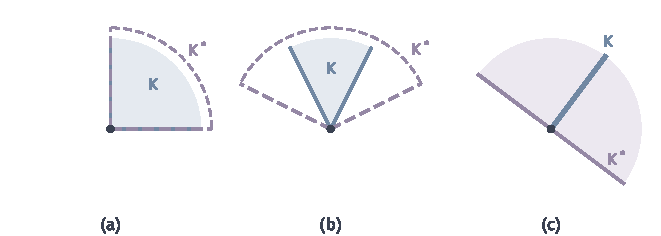
\includegraphics[width=112mm]{figures/05-optimization/06-constrained-optimization/matplotlib/cone-dual-cones/figure.pdf}
  \caption{平面上的锥（蓝色）与对偶锥（紫色）。(a)第一象限的对偶锥是它自身，紫色虚线与蓝色边界重合。(b)窄锥$\{(u,t):\lvert u\rvert\leq t/2\}$的对偶锥是宽锥$\{(v,w):\lvert v\rvert\leq2w\}$。(c)一条射线的对偶锥是一个闭半平面。各锥只画出原点附近的一部分。}
  \label{fig:cone-dual-cones}
\end{BookInlineFigure}

(b)可以手算。设$\bm{K}=\{(u,t):\lvert u\rvert\leq t/2\}$，对$(v,w)$要求$vu+wt\geq0$对所有$\bm{K}$中的点成立。固定$t\geq0$，左端在$u=\pm t/2$中使$vu$为负的那一端最小，最小值是
\[
 -\lvert v\rvert\frac{t}{2}+wt=t\Bigl(w-\frac{\lvert v\rvert}{2}\Bigr).
\]
它对所有$t\geq0$非负，当且仅当$\lvert v\rvert\leq2w$。$\bm{K}$越窄，需要照顾的方向越少，$\bm{K}^*$就越宽。

\paragraph{下界与证书}
第~\ref{chap:duality}章的做法是：把约束乘上乘子加进目标，再对$\bm{x}$取下确界，得到最优值的下界。这里用同样的计算，只是把“非负乘子”换成“对偶锥中的乘子”。

取$\bm{y}\in\mathbb{R}^p$和$\bm{s}\in\bm{K}^*$，构造
\[
 \mathcal{L}(\bm{x},\bm{y},\bm{s})=\bm{c}^\top\bm{x}+\bm{y}^\top(\bm{b}-\bm{A}\bm{x})-\bm{s}^\top(\bm{E}\bm{x}+\bm{g}).
\]
可行的$\bm{x}$满足$\bm{b}-\bm{A}\bm{x}=\bm{0}$，且$\bm{s}^\top(\bm{E}\bm{x}+\bm{g})\geq0$，所以$\mathcal{L}\leq\bm{c}^\top\bm{x}$。

$\mathcal{L}$对$\bm{x}$是仿射的，$\bm{x}$的系数必须为零，下确界才不是$-\infty$。这个条件是$\bm{A}^\top\bm{y}+\bm{E}^\top\bm{s}=\bm{c}$，此时下确界等于$\bm{b}^\top\bm{y}-\bm{g}^\top\bm{s}$。于是得到\term{锥对偶问题}（conic dual problem）
\begin{equation}
 \max_{\bm{y},\bm{s}}\ \bm{b}^\top\bm{y}-\bm{g}^\top\bm{s}\quad\text{s.t.}\quad\bm{A}^\top\bm{y}+\bm{E}^\top\bm{s}=\bm{c},\quad\bm{s}\in\bm{K}^*.
 \label{eq:cone-conic-dual}
\end{equation}

\begin{theorem}[锥规划的弱对偶]
\label{thm:cone-weak-duality}
设$\bm{x}$是问题~\eqref{eq:cone-conic}的可行点，$(\bm{y},\bm{s})$是问题~\eqref{eq:cone-conic-dual}的可行点，则
\begin{equation}
 \bm{c}^\top\bm{x}-(\bm{b}^\top\bm{y}-\bm{g}^\top\bm{s})=\bm{s}^\top(\bm{E}\bm{x}+\bm{g})\geq0.
 \label{eq:cone-conic-gap}
\end{equation}
\end{theorem}

\begin{proof}
把$\bm{c}=\bm{A}^\top\bm{y}+\bm{E}^\top\bm{s}$代入$\bm{c}^\top\bm{x}$，并用$\bm{A}\bm{x}=\bm{b}$，得到
\[
 \bm{c}^\top\bm{x}=\bm{y}^\top\bm{b}+\bm{s}^\top\bm{E}\bm{x}.
\]
两边减去$\bm{b}^\top\bm{y}-\bm{g}^\top\bm{s}$，右端成为$\bm{s}^\top(\bm{E}\bm{x}+\bm{g})$。由$\bm{s}\in\bm{K}^*$和$\bm{E}\bm{x}+\bm{g}\in\bm{K}$，它非负。
\end{proof}

式~\eqref{eq:cone-conic-gap}的用法是：手里有一个原始可行点和一个对偶可行点，最优值就被夹在两个目标值之间。若两个值相等，两个点同时最优。这个判断只用到可行性和内积，不需要知道它们是怎么算出来的。

对线性规划，$\bm{K}^*=\mathbb{R}^n_+$，问题~\eqref{eq:cone-conic-dual}就是第~\ref{chap:linear-programming}章的对偶问题，式~\eqref{eq:cone-conic-gap}就是$\bm{s}^\top\bm{x}\geq0$。

\subsection{二阶锥规划}
\label{sec:cone-socp}

“到某点的距离不超过某个值”是最常见的弯曲约束。这一小节要把它写进锥规划，并弄清右端的符号在其中起什么作用。

\paragraph{二阶锥}
距离上限的形状是一个圆盘。把半径$t$也当作变量，圆盘就随高度放大，叠起来成为一个圆锥。

\begin{definition}[二阶锥规划]
\label{def:cone-socp}
集合
\begin{equation}
 \bm{K}_{\mathrm{so}}^{k+1}=\{(\bm{u},t)\in\mathbb{R}^k\times\mathbb{R}:\lVert\bm{u}\rVert_2\leq t\}
 \label{eq:cone-soc}
\end{equation}
称为\term{二阶锥}（second-order cone）。问题
\begin{equation}
 \begin{aligned}
 \min_{\bm{x}}\quad&\bm{q}^\top\bm{x}\\
 \text{s.t.}\quad&\lVert\bm{A}_i\bm{x}+\bm{b}_i\rVert_2\leq\bm{c}_i^\top\bm{x}+d_i,\quad i=1,\ldots,m,\\
 &\bm{A}\bm{x}=\bm{b}
 \end{aligned}
 \label{eq:cone-socp}
\end{equation}
称为\term{二阶锥规划}（second-order cone program，SOCP）。这里$\bm{A}_i\in\mathbb{R}^{k_i\times n}$，$\bm{b}_i\in\mathbb{R}^{k_i}$，$\bm{c}_i\in\mathbb{R}^n$，$d_i\in\mathbb{R}$。
\end{definition}

第$i$条约束说的正是
\[
 (\bm{A}_i\bm{x}+\bm{b}_i,\ \bm{c}_i^\top\bm{x}+d_i)\in\bm{K}_{\mathrm{so}}^{k_i+1}.
\]

这个集合确实是闭凸锥。放缩时范数按倍数变化，$\theta\geq0$时仍有$\lVert\theta\bm{u}\rVert_2\leq\theta t$；相加时由三角不等式，
\[
 \lVert\bm{u}_1+\bm{u}_2\rVert_2\leq\lVert\bm{u}_1\rVert_2+\lVert\bm{u}_2\rVert_2\leq t_1+t_2.
\]
放缩和相加封闭，合起来就是凸。闭性来自范数连续。

图~\ref{fig:cone-soc-3d}画出$k=2$时的二阶锥，高度为$t$的水平截面是半径为$t$的圆盘。

\begin{BookInlineFigure}
  \centering
  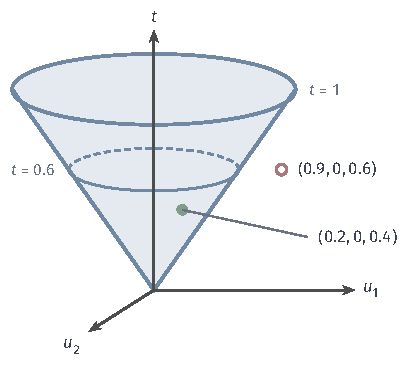
\includegraphics[width=66mm]{figures/05-optimization/06-constrained-optimization/tikz/cone-soc-3d/figure.pdf}
  \caption{$\mathbb{R}^3$中的二阶锥$\sqrt{u_1^2+u_2^2}\leq t$，画出$0\leq t\leq1$的部分。绿点$(0.2,0,0.4)$满足$0.2\leq0.4$，在锥内。红色空心点$(0.9,0,0.6)$不满足$0.9\leq0.6$，在锥外。}
  \label{fig:cone-soc-3d}
\end{BookInlineFigure}

\paragraph{右端非负也是条件的一部分}
约束的左端是范数，总是非负的，所以满足约束就迫使$\bm{c}_i^\top\bm{x}+d_i\geq0$。这个隐含的符号条件不可丢弃。

有人会想两边平方，把约束写成$\lVert\bm{u}\rVert_2^2\leq t^2$。这一步改变了集合。正确的等价关系是
\begin{equation}
 \lVert\bm{u}\rVert_2\leq t\quad\Longleftrightarrow\quad t\geq0\text{ 且 }\lVert\bm{u}\rVert_2^2\leq t^2.
 \label{eq:cone-soc-square}
\end{equation}
去掉$t\geq0$后，$(u,t)=(1,-2)$满足$1\leq4$，却不满足$1\leq-2$。

图~\ref{fig:cone-soc-square}对比了两个集合。平方之后得到的是上下两片，这个集合甚至不凸。

\begin{BookInlineFigure}
  \centering
  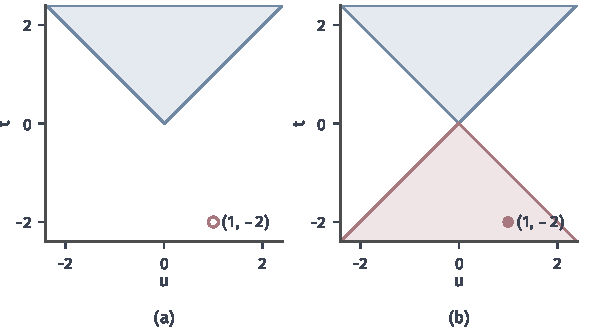
\includegraphics[width=100mm]{figures/05-optimization/06-constrained-optimization/matplotlib/cone-soc-square/figure.pdf}
  \caption{平方丢失符号信息。(a)二阶锥$\lvert u\rvert\leq t$，点$(1,-2)$不在其中。(b)$u^2\leq t^2$的解集多出了红色的下半部分，点$(1,-2)$落在其中，集合不再是凸集。}
  \label{fig:cone-soc-square}
\end{BookInlineFigure}

\paragraph{距离上限的交集}
下面用一个能手算的例子看这类可行集。在两个圆盘的公共部分里求最低的点：
\begin{equation}
 \min_{\bm{x}\in\mathbb{R}^2}\ x_2\quad\text{s.t.}\quad\lVert\bm{x}-\bm{a}_1\rVert_2\leq5,\quad\lVert\bm{x}-\bm{a}_2\rVert_2\leq5,
 \label{eq:cone-lens}
\end{equation}
其中$\bm{a}_1=(0,0)$，$\bm{a}_2=(6,0)$。对照式~\eqref{eq:cone-socp}，$\bm{q}=(0,1)$，$\bm{A}_i=\bm{I}$，$\bm{b}_i=-\bm{a}_i$，$\bm{c}_i=\bm{0}$，$d_i=5$。

每条约束是一个圆盘，二者的交仍是凸集，形状像一枚透镜，如图~\ref{fig:cone-soc-lens}所示。它的边界是弯的，所以不是多面体，线性规划和二次规划的可行集都表达不了。

\begin{BookInlineFigure}
  \centering
  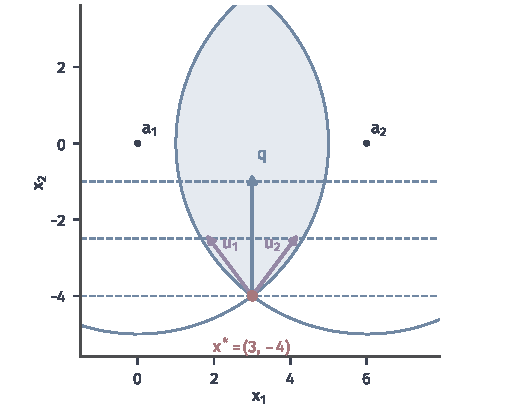
\includegraphics[width=88mm]{figures/05-optimization/06-constrained-optimization/matplotlib/cone-soc-lens/figure.pdf}
  \caption{两条距离约束的交集。浅蓝透镜是可行集，蓝色虚线是目标$x_2$的等值线，红点是解$(3,-4)$。紫色箭头是第~\ref{sec:cone-duality-certificates}小节算出的乘子分量$\bm{u}_1,\bm{u}_2$，蓝色箭头是目标系数$\bm{q}=\bm{u}_1+\bm{u}_2$，三者同乘$3.2$后画出。}
  \label{fig:cone-soc-lens}
\end{BookInlineFigure}

透镜的最低点是两个圆的交点。把两个圆的方程相减，
\[
 x_1^2+x_2^2-(x_1-6)^2-x_2^2=0,
\]
化简得$x_1=3$。代回第一个圆，得到$x_2=\pm4$。所以候选解是$(3,-4)$，目标值$-4$。它确实最优，稍后用对偶解来证明。

\paragraph{右端含变量}
约束右端也可以依赖决策变量。设要找一个位置$\bm{x}$，使它到三个站点的最大距离最小。引入变量$t$表示这个最大距离，问题写成
\begin{equation}
 \min_{\bm{x},t}\ t\quad\text{s.t.}\quad\lVert\bm{x}-\bm{p}_i\rVert_2\leq t,\quad i=1,2,3.
 \label{eq:cone-enclosing}
\end{equation}
这里决策变量是$(\bm{x},t)\in\mathbb{R}^3$，每条约束的右端$\bm{c}_i^\top(\bm{x},t)+d_i$就是$t$。在$(\bm{x},t)$空间里，每条约束是一个顶点在$(\bm{p}_i,0)$的圆锥，可行集是三个圆锥的交。

取$\bm{p}_1=(0,0)$，$\bm{p}_2=(6,0)$，$\bm{p}_3=(3,9)$。点$\bm{x}^\star=(3,4)$到三个站点的距离都是$5$，图~\ref{fig:cone-soc-enclosing}(a)是相应的覆盖圆。

\begin{BookInlineFigure}
  \centering
  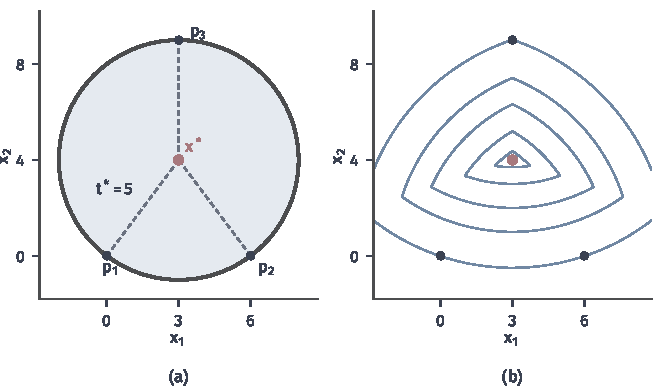
\includegraphics[width=112mm]{figures/05-optimization/06-constrained-optimization/matplotlib/cone-soc-enclosing/figure.pdf}
  \caption{最小化到三个站点的最大距离。(a)红点到三个站点的距离都等于$t^\star=5$，深灰圆是覆盖三点的最小圆。(b)蓝线是函数$\max_i\lVert\bm{x}-\bm{p}_i\rVert_2$的等高线，三段圆弧在折角处相接，目标不可微，而写成式~\eqref{eq:cone-enclosing}后目标和约束都很规则。}
  \label{fig:cone-soc-enclosing}
\end{BookInlineFigure}

下面验证$\bm{x}^\star$最优。三个站点相对$\bm{x}^\star$的位置是$(-3,-4)$、$(3,-4)$、$(0,5)$，用正权重$5,5,8$加权，和为零：
\[
 5\begin{bmatrix}-3\\-4\end{bmatrix}+5\begin{bmatrix}3\\-4\end{bmatrix}+8\begin{bmatrix}0\\5\end{bmatrix}=\bm{0}.
\]
所以对任何位移$\bm{d}\neq\bm{0}$，三个数$\bm{d}^\top(\bm{p}_i-\bm{x}^\star)$不可能全部非负且不全为零；又因三个向量张成平面，它们也不会全为零。因此总有某个$i$使$\bm{d}^\top(\bm{p}_i-\bm{x}^\star)<0$。

对这个$i$，位移后的距离满足
\[
 \lVert\bm{x}^\star+\bm{d}-\bm{p}_i\rVert_2^2=25+\lVert\bm{d}\rVert_2^2-2\bm{d}^\top(\bm{p}_i-\bm{x}^\star)>25.
\]
最大距离严格变大，所以$\bm{x}^\star$是唯一的最优位置，$t^\star=5$。

\subsection{半正定规划}
\label{sec:cone-sdp}

有些量天然是矩阵，而且必须像协方差矩阵那样半正定。这一小节回答：矩阵半正定的约束怎样放进锥规划，它能表达哪些条件，又怎样用特征值检验？

\paragraph{矩阵作变量}
记$\mathcal{S}^n$为$n\times n$实对称矩阵组成的线性空间。在其上使用\term{迹内积}（trace inner product）
\begin{equation}
 \langle\bm{X},\bm{Y}\rangle=\operatorname{tr}(\bm{X}\bm{Y})=\sum_{i,j}X_{i,j}Y_{i,j}.
 \label{eq:cone-trace-inner}
\end{equation}
把矩阵按元素排成长向量，这就是普通的欧氏内积。

半正定矩阵的集合记为$\mathcal{S}^n_+$。$\bm{X}\in\mathcal{S}^n_+$的定义是对所有$\bm{v}$有$\bm{v}^\top\bm{X}\bm{v}\geq0$，等价于全部特征值非负，这个等价关系可参考\BookChapterRef{chap:eigen-spectral-decomposition}{卷二第6章“谱分解”}。

$\mathcal{S}^n_+$是闭凸锥。对固定的$\bm{v}$，$\bm{v}^\top\bm{X}\bm{v}\geq0$是$\bm{X}$的一个线性不等式，定义的是过原点的闭半空间。$\mathcal{S}^n_+$是无穷多个这样的闭半空间的交，所以它闭、凸，且对非负放缩封闭。

\begin{definition}[半正定规划]
\label{def:cone-sdp}
给定$\bm{W},\bm{A}_1,\ldots,\bm{A}_m\in\mathcal{S}^n$和$\bm{b}\in\mathbb{R}^m$，问题
\begin{equation}
 \begin{aligned}
 \min_{\bm{X}\in\mathcal{S}^n}\quad&\langle\bm{W},\bm{X}\rangle\\
 \text{s.t.}\quad&\langle\bm{A}_i,\bm{X}\rangle=b_i,\quad i=1,\ldots,m,\\
 &\bm{X}\succeq\bm{0}
 \end{aligned}
 \label{eq:cone-sdp}
\end{equation}
称为\term{半正定规划}（semidefinite program，SDP）。$\bm{X}\succeq\bm{0}$表示$\bm{X}\in\mathcal{S}^n_+$。
\end{definition}

\paragraph{半正定不是逐元素非负}
“$\bm{X}\succeq\bm{0}$”和“$\bm{X}$的元素非负”容易混淆，其实二者互不包含。$\begin{bmatrix}1&2\\2&1\end{bmatrix}$元素全正，特征值却有$-1$。$\begin{bmatrix}1&-1\\-1&1\end{bmatrix}$有负元素，特征值是$0$和$2$，半正定。

为了看清这个差别，取迹为$1$的$2\times2$对称矩阵
\[
 \bm{X}=\begin{bmatrix}a&b\\b&1-a\end{bmatrix}.
\]
$2\times2$矩阵半正定，当且仅当两个对角元和行列式都非负。这里就是$a(1-a)-b^2\geq0$，配方得到
\[
 \Bigl(a-\frac12\Bigr)^2+b^2\leq\frac14.
\]
半正定的矩阵组成一个圆盘，而逐元素非负的要求是一条竖带的上半部分，见图~\ref{fig:cone-sdp-disk}。

\begin{BookInlineFigure}
  \centering
  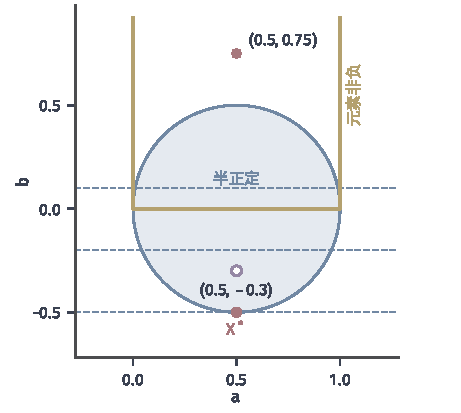
\includegraphics[width=78mm]{figures/05-optimization/06-constrained-optimization/matplotlib/cone-sdp-disk/figure.pdf}
  \caption{迹为$1$的$2\times2$对称矩阵$\begin{bmatrix}a&b\\b&1-a\end{bmatrix}$。浅蓝圆盘是半正定矩阵，黄线围住的是逐元素非负的矩阵。红色方块$(0.5,0.75)$元素非负但不半正定，紫色空心点$(0.5,-0.3)$半正定但有负元素。蓝色虚线是目标$2+2b$的等值线，红点是最优矩阵$\bm{X}^\star$。}
  \label{fig:cone-sdp-disk}
\end{BookInlineFigure}

可行集的边界是圆，所以半正定规划的最优解一般不在有限个候选的“顶点”上。在这个切片上取$\bm{W}=\begin{bmatrix}2&1\\1&2\end{bmatrix}$，最小化$\langle\bm{W},\bm{X}\rangle$，约束是$\operatorname{tr}\bm{X}=1$、$\bm{X}\succeq\bm{0}$。按式~\eqref{eq:cone-trace-inner}计算，
\[
 \langle\bm{W},\bm{X}\rangle=2a+2b+2(1-a)=2+2b.
\]
目标只依赖$b$，最小值在圆盘最低点$(a,b)=(1/2,-1/2)$取得，最优值是$1$，这正是$\bm{W}$的最小特征值。最优矩阵是
\[
 \bm{X}^\star=\frac12\begin{bmatrix}1&-1\\-1&1\end{bmatrix}.
\]

\paragraph{线性矩阵不等式}
实际问题常把变量放在矩阵的元素上，得到下面的约束：
\begin{equation}
 \bm{F}_0+x_1\bm{F}_1+\cdots+x_n\bm{F}_n\succeq\bm{0},
 \label{eq:cone-lmi}
\end{equation}
其中$\bm{F}_j\in\mathcal{S}^k$。这称为\term{线性矩阵不等式}（linear matrix inequality，LMI）。它正是式~\eqref{eq:cone-conic}中取$\bm{K}=\mathcal{S}^k_+$的情形，$\bm{E}\bm{x}+\bm{g}$是$\bm{x}$的仿射函数，取值为矩阵。

一条线性矩阵不等式可以表达弯曲的集合。例如
\[
 \bm{F}(\bm{x})=\begin{bmatrix}1+x_1&x_2\\x_2&1-x_1\end{bmatrix}
\]
的特征值是$1\pm\lVert\bm{x}\rVert_2$，所以$\bm{F}(\bm{x})\succeq\bm{0}$恰好是单位圆盘。

检验一个点是否可行，只需算特征值。取$\bm{x}=(0.6,0.6)$，特征值约为$0.152$和$1.849$，都为正，可行。取$\bm{x}=(0.8,0.8)$，最小特征值约为$-0.131$，不可行。图~\ref{fig:cone-sdp-lmi}(a)画出这两个点。

\begin{BookInlineFigure}
  \centering
  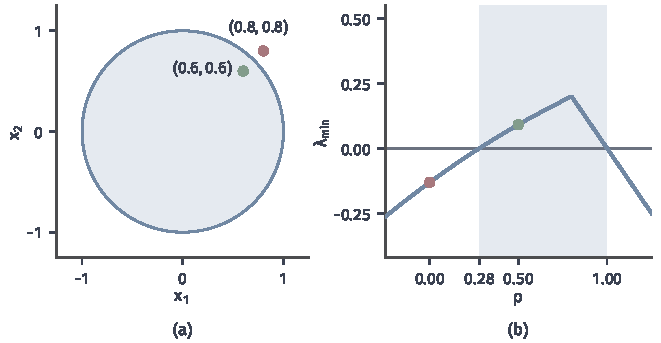
\includegraphics[width=112mm]{figures/05-optimization/06-constrained-optimization/matplotlib/cone-sdp-lmi/figure.pdf}
  \caption{用特征值检验线性矩阵不等式。(a)$\bm{F}(\bm{x})\succeq\bm{0}$的解集是单位圆盘，绿点可行，红点不可行。(b)相关矩阵~\eqref{eq:cone-corr-matrix}的最小特征值随$\rho$的变化，浅蓝区间$[0.28,1]$是使矩阵半正定的$\rho$。绿点$\rho=0.5$可行，红点$\rho=0$不可行。}
  \label{fig:cone-sdp-lmi}
\end{BookInlineFigure}

\paragraph{协方差约束}
线性矩阵不等式的一个典型来源是协方差矩阵必须半正定。设三个量两两的相关系数中，已知$\rho_{1,2}=\rho_{2,3}=0.8$，问$\rho_{1,3}=\rho$能取哪些值。相关矩阵是
\begin{equation}
 \bm{R}(\rho)=\begin{bmatrix}1&0.8&\rho\\0.8&1&0.8\\\rho&0.8&1\end{bmatrix}.
 \label{eq:cone-corr-matrix}
\end{equation}
协方差矩阵半正定这一事实的来源可参考\BookChapterRef{chap:random-vectors}{卷七第2章“随机向量与联合分布”}。这里只用到结论：$\bm{R}(\rho)$不半正定，就不存在这样的三个随机变量。

取$\rho=0$，矩阵的元素都非负，特征值却约为$-0.131$、$1$和$2.131$。所以$\rho=0$不可能，1与2强相关、2与3强相关时，1与3不能不相关。

取$\rho=0.5$，特征值约为$0.091$、$0.5$和$2.409$，可行。一般地，
\[
 \det\bm{R}(\rho)=-(\rho-1)(\rho-0.28),
\]
结合$\lvert\rho\rvert\leq1$可知可行范围是$0.28\leq\rho\leq1$，与图~\ref{fig:cone-sdp-lmi}(b)一致。

\paragraph{谱上界}
另一类重要的表达能力是控制特征值。设对称矩阵$\bm{B}(\bm{x})$仿射地依赖$\bm{x}$。对谱分解后的每个特征值看，$\lambda_{\max}(\bm{B}(\bm{x}))\leq t$等价于$t\bm{I}-\bm{B}(\bm{x})$的特征值全部非负，即
\begin{equation}
 \lambda_{\max}(\bm{B}(\bm{x}))\leq t\quad\Longleftrightarrow\quad t\bm{I}-\bm{B}(\bm{x})\succeq\bm{0}.
 \label{eq:cone-spectral-bound}
\end{equation}
所以最小化最大特征值可以写成半正定规划：在式~\eqref{eq:cone-spectral-bound}的约束下最小化$t$。

看一个具体的例子：
\[
 \bm{B}(x)=\begin{bmatrix}1+x&1\\1&3-x\end{bmatrix}.
\]
它的特征值是$2\pm\sqrt{(1-x)^2+1}$，所以$\lambda_{\max}$在$x=1$取最小值$3$。这是一个光滑例子，但$\lambda_{\max}$在特征值重合处通常不可微，而写成式~\eqref{eq:cone-spectral-bound}后，非光滑性消失在锥约束里。图~\ref{fig:cone-sdp-spectral}画出这个例子，图中的紫线下一小节解释。

\begin{BookInlineFigure}
  \centering
  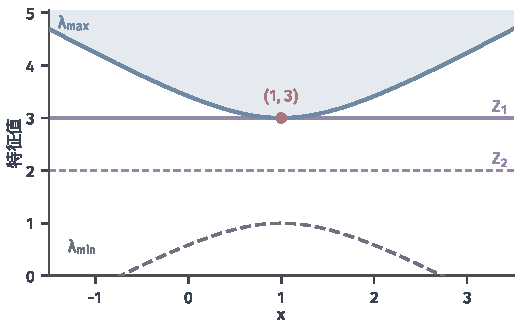
\includegraphics[width=88mm]{figures/05-optimization/06-constrained-optimization/matplotlib/cone-sdp-spectral/figure.pdf}
  \caption{$\bm{B}(x)$的两个特征值。浅蓝区域是$\lambda_{\max}(\bm{B}(x))\leq t$的$(x,t)$，红点是最优解。紫色实线$Z_1$是由$\bm{Z}_1=\frac12\begin{bmatrix}1&1\\1&1\end{bmatrix}$给出的下界$3$，紫色虚线$Z_2$是由$\bm{Z}_2=\frac12\bm{I}$给出的下界$2$。}
  \label{fig:cone-sdp-spectral}
\end{BookInlineFigure}

\subsection{锥对偶与证书}
\label{sec:cone-duality-certificates}

对偶问题~\eqref{eq:cone-conic-dual}要用到$\bm{K}^*$。这一小节算出三种常用锥的对偶锥，写出对应的对偶问题，再说明弱对偶可以放心使用，而强对偶需要额外的条件。

\paragraph{自对偶性}
下面的定理说，这三种锥的乘子就在原来的锥里取。

\begin{theorem}[三种常用锥的自对偶性]
\label{thm:cone-self-dual}
$\mathbb{R}^n_+$、$\bm{K}_{\mathrm{so}}^{k+1}$和$\mathcal{S}^n_+$的对偶锥都是它们自身。其中$\mathcal{S}^n_+$的内积取迹内积。
\end{theorem}

\begin{proof}
\emph{非负象限。}若$\bm{s}\geq\bm{0}$，对$\bm{x}\geq\bm{0}$有$\bm{s}^\top\bm{x}\geq0$。反过来，若$s_i<0$，取$\bm{x}=\bm{e}_i$得$\bm{s}^\top\bm{x}<0$。

\emph{二阶锥。}设$(\bm{v},w)$、$(\bm{u},t)$都在二阶锥中。由Cauchy--Schwarz不等式，
\[
 \bm{v}^\top\bm{u}+wt\geq-\lVert\bm{v}\rVert_2\lVert\bm{u}\rVert_2+wt\geq-wt+wt=0.
\]
所以二阶锥包含于它的对偶锥。

反过来，设$(\bm{v},w)$在对偶锥中。取$(\bm{u},t)=(\bm{0},1)$，得$w\geq0$。若$\bm{v}\neq\bm{0}$，取$\bm{u}=-\bm{v}/\lVert\bm{v}\rVert_2$、$t=1$，得到$-\lVert\bm{v}\rVert_2+w\geq0$。这两种情形都给出$\lVert\bm{v}\rVert_2\leq w$。

\emph{半正定锥。}设$\bm{X},\bm{S}\succeq\bm{0}$，由谱分解取半正定平方根，
\[
 \langle\bm{S},\bm{X}\rangle=\operatorname{tr}(\bm{S}^{1/2}\bm{X}\bm{S}^{1/2})\geq0,
\]
因为$\bm{S}^{1/2}\bm{X}\bm{S}^{1/2}$半正定，迹就是非负特征值之和。

反过来，设$\bm{S}$在对偶锥中。对任意$\bm{v}$，取$\bm{X}=\bm{v}\bm{v}^\top\succeq\bm{0}$，得到
\[
 \langle\bm{S},\bm{v}\bm{v}^\top\rangle=\bm{v}^\top\bm{S}\bm{v}\geq0,
\]
所以$\bm{S}\succeq\bm{0}$。
\end{proof}

半正定锥的乘子是半正定矩阵，不是元素非负的矩阵；二阶锥的乘子也有分量可以为负。线性规划里“乘子非负”这句话，推广之后是“乘子属于对偶锥”。

\paragraph{写出对偶问题}
把定理~\ref{thm:cone-self-dual}代入式~\eqref{eq:cone-conic-dual}。对二阶锥规划~\eqref{eq:cone-socp}，每条约束对应乘子$(\bm{u}_i,\tau_i)$，等式的乘子记作$\bm{y}$。按定义逐项写出，对偶问题是
\begin{equation}
 \begin{aligned}
 \max\quad&\bm{b}^\top\bm{y}-\sum_{i=1}^m(\bm{b}_i^\top\bm{u}_i+d_i\tau_i)\\
 \text{s.t.}\quad&\bm{A}^\top\bm{y}+\sum_{i=1}^m(\bm{A}_i^\top\bm{u}_i+\tau_i\bm{c}_i)=\bm{q},\\
 &\lVert\bm{u}_i\rVert_2\leq\tau_i,\quad i=1,\ldots,m.
 \end{aligned}
 \label{eq:cone-socp-dual}
\end{equation}

半正定规划~\eqref{eq:cone-sdp}中$\bm{X}$本身属于锥，相当于$\bm{E}$是恒等映射、$\bm{g}=\bm{0}$，对偶问题是
\begin{equation}
 \max_{\bm{y},\bm{S}}\ \bm{b}^\top\bm{y}\quad\text{s.t.}\quad\sum_{i=1}^my_i\bm{A}_i+\bm{S}=\bm{W},\quad\bm{S}\succeq\bm{0}.
 \label{eq:cone-sdp-dual}
\end{equation}
相应的间隙公式是
\begin{equation}
 \langle\bm{W},\bm{X}\rangle-\bm{b}^\top\bm{y}=\langle\bm{S},\bm{X}\rangle.
 \label{eq:cone-sdp-gap}
\end{equation}

\begin{example}[透镜问题的对偶证书]
\label{ex:cone-lens-dual}
对问题~\eqref{eq:cone-lens}，式~\eqref{eq:cone-socp-dual}成为：在$\bm{u}_1+\bm{u}_2=\bm{q}$、$\lVert\bm{u}_i\rVert_2\leq\tau_i$下最大化
\[
 \bm{a}_1^\top\bm{u}_1+\bm{a}_2^\top\bm{u}_2-5\tau_1-5\tau_2.
\]
先任取一个可行的乘子，看它给出什么下界。取$\bm{u}_1=\bm{u}_2=(0,1/2)$，$\tau_1=\tau_2=1/2$，对偶目标是$-5$。所以无论可行点是什么，$x_2\geq-5$，这个下界对，但不紧。

要使间隙为零，由式~\eqref{eq:cone-conic-gap}，每条约束的$(\bm{u}_i,\tau_i)$必须与$(\bm{x}^\star-\bm{a}_i,5)$内积为零。两个向量都在二阶锥的边界上时，这要求$\bm{u}_i$与$\bm{x}^\star-\bm{a}_i$反向，且$\lVert\bm{u}_i\rVert_2=\tau_i$。

在$\bm{x}^\star=(3,-4)$处，这给出
\[
 \bm{u}_1=\tau_1\begin{bmatrix}-3/5\\4/5\end{bmatrix},\qquad
 \bm{u}_2=\tau_2\begin{bmatrix}3/5\\4/5\end{bmatrix}.
\]
再由$\bm{u}_1+\bm{u}_2=(0,1)$，解得
\[
 \tau_1=\tau_2=\frac58,\qquad
 \bm{u}_1=\begin{bmatrix}-3/8\\1/2\end{bmatrix},\qquad
 \bm{u}_2=\begin{bmatrix}3/8\\1/2\end{bmatrix}.
\]
对偶目标是
\[
 0+\frac{18}{8}-\frac{25}{8}-\frac{25}{8}=-4.
\]
它等于原始目标值，所以$(3,-4)$最优，这对乘子也最优。图~\ref{fig:cone-soc-lens}中的紫色箭头画的就是$\bm{u}_1,\bm{u}_2$，二者之和是目标的梯度。
\end{example}

\begin{example}[谱上界的对偶证书]
\label{ex:cone-spectral-dual}
对$\min t$、$t\bm{I}-\bm{B}(x)\succeq\bm{0}$，取乘子$\bm{Z}\succeq\bm{0}$。不必套公式，直接从谱上界出发：任何$\operatorname{tr}\bm{Z}=1$的$\bm{Z}\succeq\bm{0}$都满足
\[
 \lambda_{\max}(\bm{B}(x))\geq\langle\bm{Z},\bm{B}(x)\rangle,
\]
因为$\lambda_{\max}\bm{I}-\bm{B}(x)\succeq\bm{0}$与$\bm{Z}$的迹内积非负。

若再选$\bm{Z}$使右端不含$x$，就得到一个对所有$x$成立的常数下界。$\bm{B}(x)$中$x$的系数是$\operatorname{diag}(1,-1)$，所以要求$Z_{1,1}=Z_{2,2}$，再由迹为$1$得$Z_{1,1}=Z_{2,2}=1/2$。取$Z_{1,2}=1/2$，得到
\[
 \bm{Z}_1=\frac12\begin{bmatrix}1&1\\1&1\end{bmatrix},\qquad
 \langle\bm{Z}_1,\bm{B}(x)\rangle=\frac12(1+x+2+3-x)=3.
\]
变量$x$消掉了，于是$\lambda_{\max}(\bm{B}(x))\geq3$对所有$x$成立。$x=1$时取等，这就是最优性的证明，即图~\ref{fig:cone-sdp-spectral}的紫色实线。

取$Z_{1,2}=0$，同样的计算给出常数$2$，下界正确但不紧，是图中的紫色虚线。
\end{example}

\paragraph{矩阵互补}
式~\eqref{eq:cone-conic-gap}说明，零间隙等价于$\bm{s}^\top(\bm{E}\bm{x}+\bm{g})=0$，这是互补松弛的锥形式。半正定时，这个条件比一个数等于零更强。

设$\bm{X},\bm{S}\succeq\bm{0}$且$\langle\bm{S},\bm{X}\rangle=0$，则
\[
 \operatorname{tr}(\bm{S}^{1/2}\bm{X}\bm{S}^{1/2})=\lVert\bm{X}^{1/2}\bm{S}^{1/2}\rVert_{\mathrm{F}}^2=0.
\]
所以$\bm{X}^{1/2}\bm{S}^{1/2}=\bm{0}$，再两边分别乘$\bm{X}^{1/2}$和$\bm{S}^{1/2}$，得到
\begin{equation}
 \bm{X}\bm{S}=\bm{0}.
 \label{eq:cone-matrix-complementarity}
\end{equation}
二者的列空间互相正交，秩之和不超过$n$。

以迹为$1$的例子验证。对偶问题是$\max y$、$\bm{S}=\bm{W}-y\bm{I}\succeq\bm{0}$，最优值在$y=\lambda_{\min}(\bm{W})=1$取得。这时
\[
 \bm{S}=\begin{bmatrix}1&1\\1&1\end{bmatrix},\qquad
 \bm{X}^\star\bm{S}=\frac12\begin{bmatrix}1&-1\\-1&1\end{bmatrix}\begin{bmatrix}1&1\\1&1\end{bmatrix}=\bm{0}.
\]

\paragraph{强对偶需要条件}
弱对偶无条件成立，证书就是这么来的。但两个目标值是否一定能碰到一起？线性规划中，只要原始和对偶都可行，最优值就相等且都能取到。这一结论不能原样推广。

类似第~\ref{chap:duality}章的Slater条件，锥规划也有严格可行性的条件。若存在满足$\bm{A}\bm{x}=\bm{b}$且$\bm{E}\bm{x}+\bm{g}\in\operatorname{int}\bm{K}$的点，并且原始最优值有限，则对偶问题取得最优解，且间隙为零。把原始和对偶的角色对调，结论同样成立。证明用凸集分离定理，与Slater条件的论证相同，只是把标量不等式换成锥成员条件，读者可查阅凸优化教材\scite{math-boyd2004convex}。

下面两个例子说明缺少这一条件时会出什么问题。

\begin{example}[最优值取不到]
\label{ex:cone-non-attain}
考虑
\[
 \min_{\bm{x}}\ x_1\quad\text{s.t.}\quad\begin{bmatrix}x_1&1\\1&x_2\end{bmatrix}\succeq\bm{0}.
\]
约束等价于$x_1,x_2>0$且$x_1x_2\geq1$，可行集是双曲线上方的区域，如图~\ref{fig:cone-sdp-gaps}(a)所示。取$x_1=1/k$、$x_2=k$，目标趋于$0$，但$x_1=0$不可行，最优值$0$取不到。

把式~\eqref{eq:cone-conic-dual}写出来：$\bm{Z}\succeq\bm{0}$，$Z_{1,1}=1$，$Z_{2,2}=0$，目标是$-2Z_{1,2}$。半正定和$Z_{2,2}=0$迫使$Z_{1,2}=0$，对偶唯一的可行值是$0$，它取到了。

这里原始严格可行（取$x_1=x_2=2$），所以对偶取得最优且间隙为零，符合上面的结论。对偶没有严格可行点，所以原始不保证取得最优解。
\end{example}

\begin{example}[正的对偶间隙]
\label{ex:cone-positive-gap}
考虑
\[
 \min_{\bm{x}}\ x_1\quad\text{s.t.}\quad\begin{bmatrix}0&x_1&0\\x_1&x_2&0\\0&0&x_1+1\end{bmatrix}\succeq\bm{0}.
\]
半正定矩阵的对角元为零时，同行同列都为零，所以$x_1=0$，$p^\star=0$。

对偶问题的乘子$\bm{Z}\succeq\bm{0}$要满足两个条件。$x_2$的系数给出$Z_{2,2}=0$，从而$Z_{1,2}=0$。$x_1$的系数给出$2Z_{1,2}+Z_{3,3}=1$，从而$Z_{3,3}=1$。

对偶目标是$-Z_{3,3}=-1$，所以$d^\star=-1$。原始和对偶都可行，也都取到最优值，二者却相差$1$，见图~\ref{fig:cone-sdp-gaps}(b)。原始可行集的矩阵全部奇异，严格可行性不成立。
\end{example}

\begin{BookInlineFigure}
  \centering
  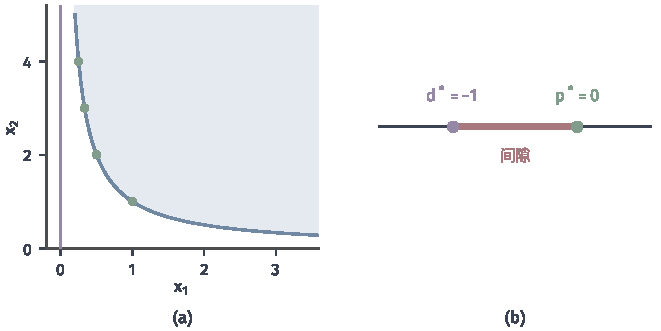
\includegraphics[width=112mm]{figures/05-optimization/06-constrained-optimization/matplotlib/cone-sdp-gaps/figure.pdf}
  \caption{半正定规划强对偶失效的两种方式。(a)浅蓝区域是可行集$x_1x_2\geq1$，绿点$(1/k,k)$的目标趋于紫线$x_1=0$，但永远到不了。(b)原始最优值$0$（绿）与对偶最优值$-1$（紫）之间有正间隙（红）。}
  \label{fig:cone-sdp-gaps}
\end{BookInlineFigure}

这些现象的根源在于，闭凸锥在线性映射下的像不一定闭。非负象限是多面体，多面体的线性像仍是闭集，二阶锥和半正定锥则没有这个保证。表~\ref{tab:cone-duality-compare}归纳了差别。

\begin{BookInlineTable}
  \centering
  \begin{tabular}{lll}
    \toprule
    性质 & 线性规划 & 一般锥规划\\
    \midrule
    弱对偶 & 成立 & 成立\\
    两边可行时间隙为零 & 成立 & 不一定\\
    最优值能取到 & 有限时取到 & 不一定\\
    零间隙的依据 & 无需额外条件 & 严格可行性等条件\\
    \bottomrule
  \end{tabular}
  \caption{线性规划与一般锥规划的对偶性质对比。}
  \label{tab:cone-duality-compare}
\end{BookInlineTable}

所以报告半正定规划的结果时，弱对偶给出的界永远可靠；“间隙为零”这句话则要么由算出的两个可行解直接验证，要么先核对严格可行性。

\section{等价改写}
\label{sec:cone-rewrite}

实际问题很少一开始就长成式~\eqref{eq:cone-qp}或式~\eqref{eq:cone-conic}的样子，常要引入辅助变量才能写进去。这就需要回答：引入辅助变量、换了约束之后，凭什么说问题没有变？

\paragraph{什么叫没有改变问题}
设原问题是在$\bm{C}$上最小化$f(\bm{x})$，改写后的问题是在$\bm{C}'$上最小化$\phi(\bm{x},\bm{z})$，其中$\bm{z}$是辅助变量。要说二者等价，需要两个方向的对应。

\begin{definition}[等价改写]
\label{def:cone-equivalent}
若下面两条都成立，则称改写后的问题是原问题的\term{等价改写}（equivalent reformulation）：
\begin{enumerate}
 \item 对每个$\bm{x}\in\bm{C}$，存在$\bm{z}$使$(\bm{x},\bm{z})\in\bm{C}'$，且$\phi(\bm{x},\bm{z})\leq f(\bm{x})$；
 \item 对每个$(\bm{x},\bm{z})\in\bm{C}'$，都有$\bm{x}\in\bm{C}$，且$f(\bm{x})\leq\phi(\bm{x},\bm{z})$。
\end{enumerate}
\end{definition}

第一条说原问题的每个候选都有替身，而且替身的代价不更高。第二条说消去辅助变量后回到的正是原约束，代价也没有被低估。

\begin{theorem}[等价改写保持最优值与最优解]
\label{thm:cone-equivalent}
在定义~\ref{def:cone-equivalent}的条件下，两个问题的最优值相等。若$(\bm{x}^\star,\bm{z}^\star)$是改写问题的最优解，则$\bm{x}^\star$是原问题的最优解。若$\bm{x}^\star$是原问题的最优解，则它配上第一条中的$\bm{z}$是改写问题的最优解。
\end{theorem}

\begin{proof}
记两个最优值为$p$和$p'$。第一条说明，原问题的每个目标值都不低于改写问题的某个目标值，于是$p'\leq p$。第二条同理给出$p\leq p'$，所以$p=p'$。

设$(\bm{x}^\star,\bm{z}^\star)$最优。第二条给出$\bm{x}^\star\in\bm{C}$，以及
\[
 f(\bm{x}^\star)\leq\phi(\bm{x}^\star,\bm{z}^\star)=p'=p.
\]
所以$\bm{x}^\star$最优。

设$\bm{x}^\star$最优，取第一条中的$\bm{z}$。则$(\bm{x}^\star,\bm{z})$可行，且
\[
 \phi(\bm{x}^\star,\bm{z})\leq f(\bm{x}^\star)=p=p'.
\]
所以它最优。
\end{proof}

定理同时给出了恢复原变量的办法：解改写问题，然后把辅助变量丢掉。对照图~\ref{fig:cone-rewrite-project}(a)，改写后的可行集沿辅助变量方向投影，恰好覆盖原可行集。

\begin{BookInlineFigure}
  \centering
  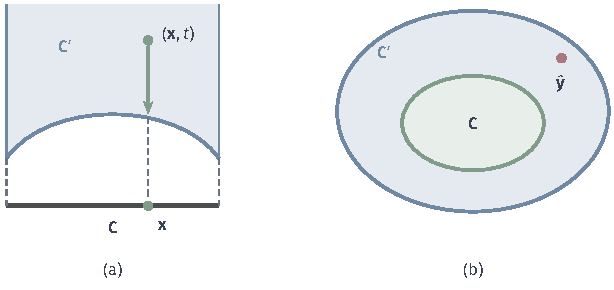
\includegraphics[width=104mm]{figures/05-optimization/06-constrained-optimization/tikz/cone-rewrite-project/figure.pdf}
  \caption{等价改写与松弛的区别。(a)等价改写：点$(\bm{x},t)$沿竖直方向下移不增加代价，投影后回到$\bm{C}$，$\bm{C}'$的投影恰是$\bm{C}$（深灰线段）。(b)松弛：$\bm{C}'$严格包含$\bm{C}$，$\bm{C}'$中可能有红点$\hat{\bm{y}}$这样不对应任何原可行点的元素，所以只保留定义中的第一条。}
  \label{fig:cone-rewrite-project}
\end{BookInlineFigure}

若只有第一条成立，得到的是另一种东西：改写后的问题最优值不超过原问题，但它的解可能不对应任何原可行点。这就是图中的(b)，留到第~\ref{sec:cone-relax}节讨论。

\subsection{上图形式}
\label{sec:cone-epigraph}

目标是非线性函数时，能否把非线性移到约束里，使目标变成线性的？这一小节用范数和凸二次两种目标回答这个问题。

\paragraph{范数目标}
函数$f$的\term{上图}（epigraph）是它图像上方的点集$\{(\bm{x},t):f(\bm{x})\leq t\}$。最小化$f$，就是在上图中寻找最低的点。

对$\min\lVert\bm{D}\bm{x}-\bm{r}\rVert_2$，引入$t$，写成
\begin{equation}
 \min_{\bm{x},t}\ t\quad\text{s.t.}\quad\lVert\bm{D}\bm{x}-\bm{r}\rVert_2\leq t.
 \label{eq:cone-norm-epigraph}
\end{equation}
目标成了线性函数，约束是一条二阶锥约束。

核对定义~\ref{def:cone-equivalent}。对任意$\bm{x}$，取$t=\lVert\bm{D}\bm{x}-\bm{r}\rVert_2$，可行，代价相等，第一条成立。对任意可行的$(\bm{x},t)$，$\lVert\bm{D}\bm{x}-\bm{r}\rVert_2\leq t$，第二条成立。

最优时约束取等号：若$t>\lVert\bm{D}\bm{x}-\bm{r}\rVert_2$，把$t$减小到等号处仍可行，目标更低。图~\ref{fig:cone-epigraph}(a)中的绿色箭头就是这个下移。

\begin{BookInlineFigure}
  \centering
  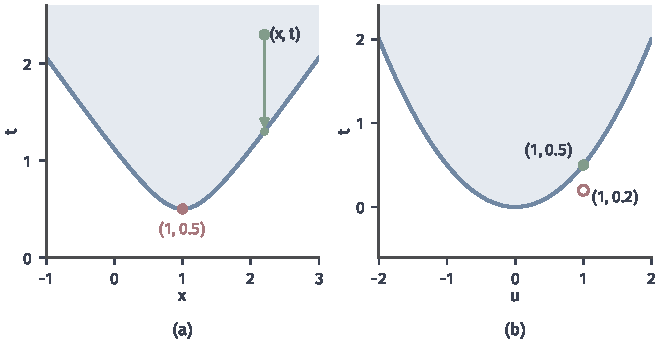
\includegraphics[width=112mm]{figures/05-optimization/06-constrained-optimization/matplotlib/cone-epigraph/figure.pdf}
  \caption{上图改写。(a)$f(x)=\lVert(x-1,1/2)\rVert_2$的上图（浅蓝），绿点下移到函数图像上时$t$减小而$x$不变，红点是上图中的最低点。(b)在网格上逐点判定$\lVert(2u,2t-1)\rVert_2\leq2t+1$，浅蓝区域恰是抛物线$t\geq u^2/2$的上方，绿点$(1,0.5)$在边界上，红色空心点$(1,0.2)$不满足约束。}
  \label{fig:cone-epigraph}
\end{BookInlineFigure}

\paragraph{凸二次目标}
平方范数多了一层：$\frac12\bm{x}^\top\bm{Q}\bm{x}\leq t$的左端是二次的，不是范数。这需要两步转换。

第一步是分解。$\bm{Q}\succeq\bm{0}$时存在$\bm{F}\in\mathbb{R}^{k\times n}$使$\bm{Q}=\bm{F}^\top\bm{F}$，例如取Cholesky因子或由谱分解得到。最小二乘中直接有$\bm{F}=\bm{D}$。于是上图约束是$\lVert\bm{F}\bm{x}\rVert_2^2\leq2t$。

第二步把“平方范数不超过乘积”写成二阶锥。

\begin{lemma}[旋转二阶锥]
\label{lem:cone-rotated-soc}
对$\bm{u}\in\mathbb{R}^k$和$s,w\in\mathbb{R}$，
\begin{equation}
 \lVert\bm{u}\rVert_2^2\leq sw,\quad s\geq0,\quad w\geq0
 \quad\Longleftrightarrow\quad
 \left\lVert\begin{bmatrix}2\bm{u}\\s-w\end{bmatrix}\right\rVert_2\leq s+w.
 \label{eq:cone-rotated-soc}
\end{equation}
\end{lemma}

\begin{proof}
先证从左到右。由$\lVert\bm{u}\rVert_2^2\leq sw$，
\[
 4\lVert\bm{u}\rVert_2^2+(s-w)^2\leq4sw+(s-w)^2=(s+w)^2.
\]
又$s+w\geq0$，两边开方得到右式。

再证从右到左。右式的范数不小于$\lvert s-w\rvert$，所以$s+w\geq\lvert s-w\rvert$。分别取绝对值的两种符号，得到$w\geq0$和$s\geq0$。把右式平方，同样的展开给出$4\lVert\bm{u}\rVert_2^2\leq4sw$。
\end{proof}

取$\bm{u}=\bm{F}\bm{x}$、$s=2t$、$w=1$，就得到$\lVert\bm{F}\bm{x}\rVert_2^2\leq2t$的二阶锥形式。凸二次规划~\eqref{eq:cone-qp}因而等价于
\begin{equation}
 \begin{aligned}
 \min_{\bm{x},t}\quad&t+\bm{q}^\top\bm{x}\\
 \text{s.t.}\quad&\left\lVert\begin{bmatrix}2\bm{F}\bm{x}\\2t-1\end{bmatrix}\right\rVert_2\leq2t+1,\\
 &\bm{A}\bm{x}=\bm{b},\quad\bm{G}\bm{x}\leq\bm{h}.
 \end{aligned}
 \label{eq:cone-qp-socp}
\end{equation}
图~\ref{fig:cone-epigraph}(b)用网格判定的方式核对了$k=1$的情形：约束$\lVert(2u,2t-1)\rVert_2\leq2t+1$的解集正好是$t\geq u^2/2$。

再用定义~\ref{def:cone-equivalent}核对。第一条取$t=\frac12\bm{x}^\top\bm{Q}\bm{x}$。第二条由引理得到$t\geq\frac12\bm{x}^\top\bm{Q}\bm{x}$，于是原目标不超过改写后的目标。恢复$\bm{x}$时丢弃$t$即可。

\begin{example}[预算问题的二阶锥形式]
\label{ex:cone-budget-socp}
预算问题的目标是$\frac12\lVert\bm{D}\bm{x}-\bm{r}\rVert_2^2$，这里取$\bm{u}=\bm{D}\bm{x}-\bm{r}$，约束写成
\[
 \left\lVert\begin{bmatrix}2(\bm{D}\bm{x}-\bm{r})\\2t-1\end{bmatrix}\right\rVert_2\leq2t+1.
\]
在$\bm{x}^\star=(3/2,1/2)$处，残差是$(-2,1/2,1/2)$，取$t=9/4$。左端向量是$(-4,1,1,7/2)$，长度的平方是
\[
 16+1+1+\frac{49}{4}=\frac{121}{4}.
\]
所以左端等于$11/2$，右端也等于$2t+1=11/2$。约束取等号，改写问题的目标值$t=9/4$与原问题的$f^\star$相同。
\end{example}

只有$\bm{Q}\succeq\bm{0}$时才有实分解$\bm{Q}=\bm{F}^\top\bm{F}$。第~\ref{sec:cone-nonconvex-qp}小节的$\operatorname{diag}(1,-1)$没有这样的分解，也不可能写成式~\eqref{eq:cone-qp-socp}：二阶锥规划的可行集是凸的，而目标的上图不凸。

另外，若目标是$\min\lVert\bm{D}\bm{x}-\bm{r}\rVert_2^2$，也可以直接最小化不带平方的范数。平方在非负数上严格递增，所以两者最优解相同；但最优值不同，这与定义~\ref{def:cone-equivalent}的“最优值相等”不是一回事，恢复目标值时要重新平方。

\paragraph{维数与成本}
增加变量并不自动带来计算上的好处。表~\ref{tab:cone-epi-cost}比较凸二次目标的两种写法，$\bm{Q}=\bm{F}^\top\bm{F}$，$\bm{F}\in\mathbb{R}^{k\times n}$。

\begin{BookInlineTable}
  \centering
  \begin{tabular}{lll}
    \toprule
    & 二次规划形式 & 二阶锥形式\\
    \midrule
    变量个数 & $n$ & $n+1$\\
    非线性结构 & 目标中的$\bm{Q}$ & 一个$k+2$维的二阶锥\\
    需要的准备 & $\bm{Q}$或矩阵向量积 & 分解$\bm{F}$\\
    可用的方法 & 二次规划专用方法 & 通用锥规划方法\\
    \bottomrule
  \end{tabular}
  \caption{同一凸二次目标的两种写法。}
  \label{tab:cone-epi-cost}
\end{BookInlineTable}

$\bm{Q}$稀疏时，分解因子$\bm{F}$可能比$\bm{Q}$稠密得多，改写后存储反而增加。$\bm{Q}$只能通过矩阵向量积访问时，分解根本做不出来。反过来，$\bm{Q}=\bm{D}^\top\bm{D}$稠密而$\bm{D}$稀疏时，直接用$\bm{F}=\bm{D}$比存$\bm{Q}$便宜。

改写的价值在于让问题能交给统一的求解方法，能和其他范数约束混用。只有二次目标和线性约束时，保留原形式通常更省。

\subsection{Schur补改写}
\label{sec:cone-schur}

二次上界和矩阵的逆都不是矩阵元素的线性函数。这一小节回答：这种限制能否写成线性矩阵不等式？工具是Schur补，关键是分清哪一块必须正定。

\paragraph{从配方到判据}
先看$2\times2$的情形。设$p>0$，考虑二次型
\[
 pa^2+2nab+Tb^2.
\]
配方得到
\[
 p\Bigl(a+\frac{n}{p}b\Bigr)^2+\Bigl(T-\frac{n^2}{p}\Bigr)b^2.
\]
第一项可以用$a$消成零，所以整个二次型非负，取决于第二项的系数$T-n^2/p$是否非负。

矩阵版本完全类似，只是把除以$p$换成乘以逆矩阵。

\begin{lemma}[Schur补判据]
\label{lem:cone-schur}
设对称矩阵分块为
\begin{equation}
 \bm{M}=\begin{bmatrix}\bm{P}&\bm{N}\\\bm{N}^\top&\bm{T}\end{bmatrix},
 \label{eq:cone-block-matrix}
\end{equation}
其中$\bm{P}\succ\bm{0}$。则
\begin{equation}
 \bm{M}\succeq\bm{0}\quad\Longleftrightarrow\quad\bm{T}-\bm{N}^\top\bm{P}^{-1}\bm{N}\succeq\bm{0}.
 \label{eq:cone-schur}
\end{equation}
矩阵$\bm{T}-\bm{N}^\top\bm{P}^{-1}\bm{N}$称为$\bm{P}$在$\bm{M}$中的\term{Schur补}（Schur complement）。
\end{lemma}

\begin{proof}
对任意向量$\bm{a},\bm{b}$，记$\bm{S}=\bm{T}-\bm{N}^\top\bm{P}^{-1}\bm{N}$。配方得到
\[
 \begin{bmatrix}\bm{a}\\\bm{b}\end{bmatrix}^\top\bm{M}\begin{bmatrix}\bm{a}\\\bm{b}\end{bmatrix}
 =(\bm{a}+\bm{P}^{-1}\bm{N}\bm{b})^\top\bm{P}(\bm{a}+\bm{P}^{-1}\bm{N}\bm{b})+\bm{b}^\top\bm{S}\bm{b}.
\]
若$\bm{S}\succeq\bm{0}$，右端两项都非负，$\bm{M}\succeq\bm{0}$。

反过来，设$\bm{M}\succeq\bm{0}$。对任意$\bm{b}$，取$\bm{a}=-\bm{P}^{-1}\bm{N}\bm{b}$，第一项变为零，于是$\bm{b}^\top\bm{S}\bm{b}\geq0$。
\end{proof}

式~\eqref{eq:cone-schur}的左端对$\bm{P},\bm{N},\bm{T}$是线性的，右端含有逆和乘积。这就是改写的用处：把弯曲的右端换成线性的左端。

\paragraph{二次型上界}
令$\bm{P}=\bm{I}$、$\bm{N}=\bm{u}$、$\bm{T}=t$，由引理~\ref{lem:cone-schur}，
\begin{equation}
 \lVert\bm{u}\rVert_2^2\leq t\quad\Longleftrightarrow\quad\begin{bmatrix}\bm{I}&\bm{u}\\\bm{u}^\top&t\end{bmatrix}\succeq\bm{0}.
 \label{eq:cone-schur-quadratic}
\end{equation}
代入$\bm{u}=\bm{D}\bm{x}-\bm{r}$，左端对$\bm{x}$是二次的，右端的矩阵对$(\bm{x},t)$却是仿射的。这条约束就是一条线性矩阵不等式，和式~\eqref{eq:cone-lmi}同型。这里单位块$\bm{I}$恒正定，引理的条件自动满足。

以预算问题的解为例，$\lVert\bm{u}\rVert_2^2=9/2$。取$t=9/2$，矩阵是$4\times4$的，它的Schur补为零，矩阵半正定且奇异。取$t$更小，Schur补为负，矩阵不再半正定。

\paragraph{含逆矩阵的限制}
再看一个$\bm{P}$本身是变量的例子。设$\bm{Y}\succ\bm{0}$是对称矩阵变量，$\bm{b}$是向量，由引理~\ref{lem:cone-schur}，
\begin{equation}
 \bm{b}^\top\bm{Y}^{-1}\bm{b}\leq t\quad\Longleftrightarrow\quad\begin{bmatrix}\bm{Y}&\bm{b}\\\bm{b}^\top&t\end{bmatrix}\succeq\bm{0}\qquad(\bm{Y}\succ\bm{0}).
 \label{eq:cone-schur-inverse}
\end{equation}
右端是$(\bm{Y},\bm{b},t)$的线性矩阵不等式，也说明左端的函数在$\bm{Y}\succ\bm{0}$上对$(\bm{Y},\bm{b})$联合凸：它的上图由一条线性矩阵不等式定义。

用数值走一遍。取
\[
 \bm{Y}=\begin{bmatrix}2&1\\1&2\end{bmatrix},\qquad\bm{b}=\begin{bmatrix}1\\1\end{bmatrix}.
\]
矩阵的逆是
\[
 \bm{Y}^{-1}=\frac13\begin{bmatrix}2&-1\\-1&2\end{bmatrix}.
\]
代入得到
\[
 \bm{b}^\top\bm{Y}^{-1}\bm{b}=\frac13(2-1-1+2)=\frac23.
\]
$3\times3$块矩阵的行列式等于$\det\bm{Y}$与Schur补的乘积，
\[
 \det\bm{M}=3\Bigl(t-\frac23\Bigr).
\]
于是$t<2/3$时矩阵不半正定，$t=2/3$时恰好在边界上。数值上，$t=1/2$时最小特征值约为$-0.137$，$t=1$时约为$0.268$。图~\ref{fig:cone-schur}(a)画出最小特征值穿过零点的过程。

\begin{BookInlineFigure}
  \centering
  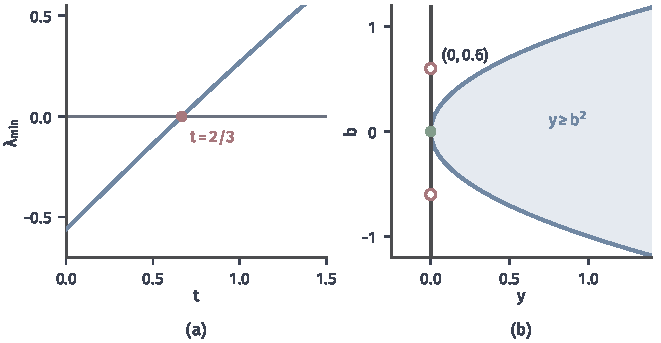
\includegraphics[width=112mm]{figures/05-optimization/06-constrained-optimization/matplotlib/cone-schur/figure.pdf}
  \caption{Schur补判据及其边界。(a)式~\eqref{eq:cone-schur-inverse}的块矩阵的最小特征值随$t$的变化，红点是$t=2/3$。(b)$\begin{bmatrix}y&b\\b&1\end{bmatrix}\succeq\bm{0}$的解集（浅蓝）是抛物线$y\geq b^2$的内部及边界。深灰线$y=0$上只有绿点$(0,0)$可行，红色空心点$(0,\pm0.6)$不可行。}
  \label{fig:cone-schur}
\end{BookInlineFigure}

\paragraph{奇异的情形}
$\bm{P}$只半正定时，不能写$\bm{P}^{-1}$，把逆换成伪逆也不够。看一个例子：
\[
 \begin{bmatrix}0&1\\1&1\end{bmatrix}.
\]
这里$\bm{P}=0$，伪逆也是$0$，“Schur补”算出来是$1\geq0$。但矩阵的行列式是$-1$，它不半正定。缺的是一个像空间的条件：$\bm{P}$的零方向上，$\bm{N}$也必须为零。

\begin{lemma}[奇异情形的Schur补判据]
\label{lem:cone-schur-singular}
在引理~\ref{lem:cone-schur}的分块中，设$\bm{P}\succeq\bm{0}$，$\bm{P}^\dagger$是其伪逆。则$\bm{M}\succeq\bm{0}$，当且仅当
\begin{equation}
 (\bm{I}-\bm{P}\bm{P}^\dagger)\bm{N}=\bm{0}\quad\text{且}\quad\bm{T}-\bm{N}^\top\bm{P}^\dagger\bm{N}\succeq\bm{0}.
 \label{eq:cone-schur-singular}
\end{equation}
\end{lemma}

\begin{proof}
设$\bm{M}\succeq\bm{0}$。任取$\bm{w}\in\ker\bm{P}$和向量$\bm{v}$，把$\bm{M}$的二次型作用在$(\bm{w},\varepsilon\bm{v})$上，得到
\[
 2\varepsilon\bm{w}^\top\bm{N}\bm{v}+\varepsilon^2\bm{v}^\top\bm{T}\bm{v}\geq0.
\]
这对正负的小$\varepsilon$都成立，必有$\bm{w}^\top\bm{N}\bm{v}=0$。所以$\bm{N}$的列与$\ker\bm{P}$正交，属于$\operatorname{range}\bm{P}$，这正是$\bm{P}\bm{P}^\dagger\bm{N}=\bm{N}$。

在条件$\bm{P}\bm{P}^\dagger\bm{N}=\bm{N}$之下，令
\[
 \bm{U}=\begin{bmatrix}\bm{I}&-\bm{P}^\dagger\bm{N}\\\bm{0}&\bm{I}\end{bmatrix},
\]
它可逆。直接相乘，并用$\bm{P}^\dagger\bm{P}\bm{P}^\dagger=\bm{P}^\dagger$，得到
\[
 \bm{U}^\top\bm{M}\bm{U}=\begin{bmatrix}\bm{P}&\bm{0}\\\bm{0}&\bm{T}-\bm{N}^\top\bm{P}^\dagger\bm{N}\end{bmatrix}.
\]
可逆合同变换保持半正定性，所以$\bm{M}\succeq\bm{0}$当且仅当右端半正定，也就是第二个条件成立。这同时完成了两个方向的证明。
\end{proof}

图~\ref{fig:cone-schur}(b)展示了这个条件的几何含义。$\begin{bmatrix}y&b\\b&1\end{bmatrix}\succeq\bm{0}$在$y>0$时等价于$b^2/y\leq1$，即$y\geq b^2$。到$y=0$时，$b^2/y$没有定义，判据要求$b=0$，图中只有原点留下。

这里还有一个定义域的问题。式~\eqref{eq:cone-schur-inverse}要求$\bm{Y}\succ\bm{0}$，而块矩阵半正定只推出$\bm{Y}\succeq\bm{0}$。改写时若丢掉严格正定的要求，集合就多了边界上的奇异$\bm{Y}$，这些点在原问题中$\bm{Y}^{-1}$并无定义。这时要么说明原函数在边界上取什么值，要么在求解后核对$\bm{Y}$是否真的正定。

\paragraph{二阶锥也是线性矩阵不等式}
同样的工具给出
\begin{equation}
 \lVert\bm{u}\rVert_2\leq t\quad\Longleftrightarrow\quad\begin{bmatrix}t\bm{I}&\bm{u}\\\bm{u}^\top&t\end{bmatrix}\succeq\bm{0}.
 \label{eq:cone-soc-as-lmi}
\end{equation}
$t>0$时由引理~\ref{lem:cone-schur}，Schur补是$t-\bm{u}^\top\bm{u}/t$。$t=0$时左上块为零，由引理~\ref{lem:cone-schur-singular}迫使$\bm{u}=\bm{0}$。$t<0$时对角元为负，矩阵不半正定。三种情形都与左式一致。

所以二阶锥规划可以写成半正定规划。这种包含关系的计算含义留到第~\ref{sec:cone-methods}节讨论。

\section{半正定松弛}
\label{sec:cone-relax}

第~\ref{sec:cone-nonconvex-qp}小节的问题不能等价地改写成凸问题，KKT条件也给不出全局证书。既然改不成凸问题，能否算出一个有保证的下界，用它判断手上的候选解离最优还有多远？

\paragraph{把乘积收集到矩阵里}
考虑\term{二次约束二次规划}（quadratically constrained quadratic program，QCQP）
\begin{equation}
 \begin{aligned}
 \min_{\bm{x}\in\mathbb{R}^n}\quad&\bm{x}^\top\bm{Q}_0\bm{x}+2\bm{q}_0^\top\bm{x}+c_0\\
 \text{s.t.}\quad&\bm{x}^\top\bm{Q}_i\bm{x}+2\bm{q}_i^\top\bm{x}+c_i\leq0,\quad i=1,\ldots,m,
 \end{aligned}
 \label{eq:cone-qcqp}
\end{equation}
其中$\bm{Q}_i$对称，可以不定。等式约束可以拆成两条不等式，因此这里只写不等式。

难点全在乘积$x_ix_j$上。这些乘积在$\bm{x}$上是非线性的，但只要把它们看成新的未知数，每个二次式都变成新未知数的线性函数。这就像把一笔难算的账换一种记法：先不管各项之间的关系，只把用到的项登记下来，账立刻变成加法。这个类比的边界是：各项之间的关系并没有消失，它们藏在下面矩阵的结构里，后面要单独处理。

具体做法是引入带常数坐标的矩阵
\begin{equation}
 \bm{Y}=\begin{bmatrix}1\\\bm{x}\end{bmatrix}\begin{bmatrix}1\\\bm{x}\end{bmatrix}^\top=\begin{bmatrix}1&\bm{x}^\top\\\bm{x}&\bm{x}\bm{x}^\top\end{bmatrix}\in\mathcal{S}^{n+1},
 \label{eq:cone-lift-matrix}
\end{equation}
行列下标从$0$开始。常数坐标的作用是把线性项和常数项也放进矩阵。记
\[
 \bm{M}_i=\begin{bmatrix}c_i&\bm{q}_i^\top\\\bm{q}_i&\bm{Q}_i\end{bmatrix},
\]
直接展开迹内积，得到
\begin{equation}
 \bm{x}^\top\bm{Q}_i\bm{x}+2\bm{q}_i^\top\bm{x}+c_i=\langle\bm{M}_i,\bm{Y}\rangle.
 \label{eq:cone-lift-linear}
\end{equation}
原来的二次式成了$\bm{Y}$的线性函数。

图~\ref{fig:cone-lift}以式~\eqref{eq:cone-nonconvex-objective}为例。这时$\bm{Q}_0=\operatorname{diag}(1/2,-1/2)$，$\bm{q}_0=(0,1/8)$，$c_0=0$。

\begin{BookInlineFigure}
  \centering
  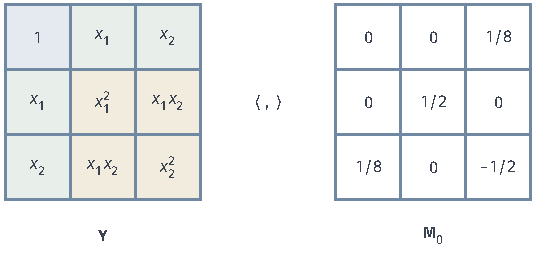
\includegraphics[width=90mm]{figures/05-optimization/06-constrained-optimization/tikz/cone-lift/figure.pdf}
  \caption{提升矩阵与目标系数。左边是$n=2$时的$\bm{Y}$，浅蓝格是常数，绿格是一次项，黄格是二次项。右边是目标$\frac12x_1^2-\frac12x_2^2+\frac14x_2$对应的$\bm{M}_0$，交叉项的系数对半分在两个对称位置上。二者的迹内积就是目标。}
  \label{fig:cone-lift}
\end{BookInlineFigure}

\paragraph{哪些矩阵来自向量}
不是每个矩阵都有式~\eqref{eq:cone-lift-matrix}的形状。下面的引理精确地指出需要哪些条件。

\begin{lemma}[秩一刻画]
\label{lem:cone-rank-one}
$\bm{Y}\in\mathcal{S}^{n+1}$具有式~\eqref{eq:cone-lift-matrix}的形状，当且仅当
\begin{equation}
 \bm{Y}\succeq\bm{0},\qquad Y_{0,0}=1,\qquad\operatorname{rank}\bm{Y}=1.
 \label{eq:cone-rank-one}
\end{equation}
\end{lemma}

\begin{proof}
式~\eqref{eq:cone-lift-matrix}的矩阵满足这三条：它是一个向量与自身的外积，秩为一且半正定，第一个元素是$1$。反过来，秩一半正定矩阵可以写成$\bm{Y}=\bm{v}\bm{v}^\top$。由$Y_{0,0}=v_0^2=1$得$v_0=\pm1$，必要时把$\bm{v}$换成$-\bm{v}$，可设$v_0=1$。记$\bm{v}=(1,\bm{x})$，$\bm{Y}$就有所要的形状。
\end{proof}

于是问题~\eqref{eq:cone-qcqp}等价于在条件~\eqref{eq:cone-rank-one}和$\langle\bm{M}_i,\bm{Y}\rangle\leq0$下最小化$\langle\bm{M}_0,\bm{Y}\rangle$。目标和约束都是线性的，半正定和$Y_{0,0}=1$也是凸约束，全部困难集中在秩一这一条上。

把它删掉，就得到\term{半正定松弛}（semidefinite relaxation）
\begin{equation}
 \begin{aligned}
 \min_{\bm{Y}\in\mathcal{S}^{n+1}}\quad&\langle\bm{M}_0,\bm{Y}\rangle\\
 \text{s.t.}\quad&\langle\bm{M}_i,\bm{Y}\rangle\leq0,\quad i=1,\ldots,m,\\
 &Y_{0,0}=1,\quad\bm{Y}\succeq\bm{0}.
 \end{aligned}
 \label{eq:cone-sdr}
\end{equation}

\subsection{松弛下界}
\label{sec:cone-relax-bound}

删掉一个约束，最优值只会变小。这一小节要把这件事写准确，并弄清楚上面的几步各自改变了什么。

\begin{theorem}[松弛给出下界]
\label{thm:cone-sdr-bound}
记问题~\eqref{eq:cone-qcqp}的最优值为$f^\star$，问题~\eqref{eq:cone-sdr}的最优值为$p_{\mathrm{rel}}$。则
\begin{equation}
 p_{\mathrm{rel}}\leq f^\star.
 \label{eq:cone-sdr-bound}
\end{equation}
\end{theorem}

\begin{proof}
任取问题~\eqref{eq:cone-qcqp}的可行点$\bm{x}$，按式~\eqref{eq:cone-lift-matrix}构造$\bm{Y}$。由引理~\ref{lem:cone-rank-one}，$\bm{Y}\succeq\bm{0}$且$Y_{0,0}=1$。由式~\eqref{eq:cone-lift-linear}，$\langle\bm{M}_i,\bm{Y}\rangle\leq0$，且$\langle\bm{M}_0,\bm{Y}\rangle$等于原目标值。所以$\bm{Y}$对问题~\eqref{eq:cone-sdr}可行，$p_{\mathrm{rel}}$不超过原目标值。对所有可行$\bm{x}$取下确界，即得结论。
\end{proof}

这个结论只用到定义~\ref{def:cone-equivalent}的第一条。第二条在这里不成立，因为松弛问题的可行矩阵不一定对应任何$\bm{x}$。表~\ref{tab:cone-relax-steps}把三步分开。

\begin{BookInlineTable}
  \centering
  \begin{tabular}{lll}
    \toprule
    步骤 & 做了什么 & 与原问题的关系\\
    \midrule
    提升 & 用$\bm{Y}$表示乘积，保留秩一 & 等价\\
    放松秩约束 & 删去$\operatorname{rank}\bm{Y}=1$ & 可行集变大，得到下界\\
    求解松弛 & 数值计算SDP & 近似解，下界需验证\\
    \bottomrule
  \end{tabular}
  \caption{半正定松弛的三个步骤。只有第一步不改变问题。}
  \label{tab:cone-relax-steps}
\end{BookInlineTable}

\begin{example}[松弛证明全局最优]
\label{ex:cone-relax-nonconvex}
回到目标~\eqref{eq:cone-nonconvex-objective}。可行集$-1\leq x_2\leq1$写成二次约束$x_2^2\leq1$。记$\bm{Y}$的元素
\[
 \bm{Y}=\begin{bmatrix}1&y_1&y_2\\y_1&X_{1,1}&X_{1,2}\\y_2&X_{1,2}&X_{2,2}\end{bmatrix}.
\]
松弛问题是在$X_{2,2}\leq1$、$\bm{Y}\succeq\bm{0}$下最小化
\[
 \frac12X_{1,1}-\frac12X_{2,2}+\frac14y_2.
\]

下面逐项估计目标。半正定矩阵的对角元非负，所以$X_{1,1}\geq0$。约束给出$X_{2,2}\leq1$。再由$\{0,2\}$行列对应的$2\times2$主子式非负，$y_2^2\leq X_{2,2}\leq1$，所以$y_2\geq-1$。三项合起来，
\[
 \frac12X_{1,1}-\frac12X_{2,2}+\frac14y_2\geq0-\frac12-\frac14=-\frac34.
\]
这个下界由点A对应的秩一矩阵取到，所以$p_{\mathrm{rel}}=-3/4$，也就是$f^\star=-3/4$。KKT条件区分不开A和B，松弛却直接证明了A是全局最优，而B的目标值$-1/4$高于下界，不是全局最优。
\end{example}

\paragraph{符号变量}
下面这个问题里，松弛一般不紧。设$\bm{W}\in\mathcal{S}^n$，考虑
\begin{equation}
 \min_{\bm{x}}\ \bm{x}^\top\bm{W}\bm{x}\quad\text{s.t.}\quad x_i^2=1,\quad i=1,\ldots,n.
 \label{eq:cone-sign-problem}
\end{equation}
变量只能取$\pm1$，这是一个把点分到两侧的组合问题。约束$x_i^2=1$恰好是二次的，提升后成为对角线上的线性条件，一条也不丢。

这里没有线性项，$\bm{Y}$中的$\bm{x}$块可以去掉。设$\bm{Y}$可行，记其$\bm{x}$块为$\hat{\bm{x}}$，令$\bm{D}_{\pm}=\operatorname{diag}(1,-\bm{I})$。矩阵$\bm{D}_{\pm}\bm{Y}\bm{D}_{\pm}$也可行，目标不变，只是$\hat{\bm{x}}$变号。二者的平均仍可行，而$\bm{x}$块为零。所以只需保留右下块$\bm{X}=\bm{x}\bm{x}^\top$，松弛写成
\begin{equation}
 \min_{\bm{X}\in\mathcal{S}^n}\ \langle\bm{W},\bm{X}\rangle\quad\text{s.t.}\quad X_{i,i}=1,\quad i=1,\ldots,n,\quad\bm{X}\succeq\bm{0}.
 \label{eq:cone-sign-relax}
\end{equation}
取$\bm{A}_i=\bm{e}_i\bm{e}_i^\top$、$b_i=1$，由式~\eqref{eq:cone-sdp-dual}，它的对偶问题是
\begin{equation}
 \max_{\bm{y}\in\mathbb{R}^n}\ \sum_{i=1}^ny_i\quad\text{s.t.}\quad\bm{W}-\operatorname{diag}(\bm{y})\succeq\bm{0}.
 \label{eq:cone-sign-dual}
\end{equation}

先看$n=2$，$\bm{W}$的对角元为零、非对角元为$1$。松弛的可行矩阵是$\begin{bmatrix}1&a\\a&1\end{bmatrix}$，$a\in[-1,1]$，目标是$2a$。最优在$a=-1$取到，矩阵秩一，对应$\bm{x}=(1,-1)$，松弛是紧的。

再看三角形的例子。取$n=3$，
\[
 \bm{W}=\begin{bmatrix}0&1&1\\1&0&1\\1&1&0\end{bmatrix}.
\]
目标是$2(x_1x_2+x_1x_3+x_2x_3)$。枚举$8$个符号组合，全同时目标为$6$，其余都是两个相同、一个相反，目标为$-2$。所以$f^\star=-2$。

松弛问题中取
\[
 \hat{\bm{X}}=\begin{bmatrix}1&-1/2&-1/2\\-1/2&1&-1/2\\-1/2&-1/2&1\end{bmatrix}.
\]
它的特征值是$0,3/2,3/2$，半正定，对角元都是$1$，所以松弛可行。六个非对角元各贡献$-1/2$，目标是
\[
 \langle\bm{W},\hat{\bm{X}}\rangle=-3.
\]

再看对偶问题~\eqref{eq:cone-sign-dual}。取$\bm{y}=(-1,-1,-1)$，则
\[
 \bm{W}-\operatorname{diag}(\bm{y})=\bm{W}+\bm{I}=\bm{1}\bm{1}^\top\succeq\bm{0},
\]
对偶目标是$-3$。原始和对偶的值相等，所以$p_{\mathrm{rel}}=-3$。

下界$-3$比真实最优值$-2$低了$1$，这个间隙来自放松秩约束，而不是求解误差。图~\ref{fig:cone-relax-slice}在切片上画出了可行集究竟扩大了多少。

\begin{BookInlineFigure}
  \centering
  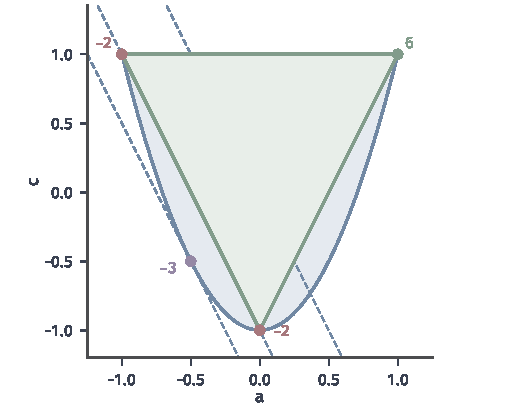
\includegraphics[width=88mm]{figures/05-optimization/06-constrained-optimization/matplotlib/cone-relax-slice/figure.pdf}
  \caption{$n=3$时松弛可行集在切片$X_{1,2}=X_{1,3}=a$、$X_{2,3}=c$上的形状。浅蓝抛物线区域$2a^2-1\leq c\leq1$是松弛的可行集。绿色三角形是秩一矩阵（符号解）的凸包，其顶点旁标注目标$4a+2c$的值。蓝色虚线是等值线，紫点是松弛最优解，目标$-3$，它在三角形之外。}
  \label{fig:cone-relax-slice}
\end{BookInlineFigure}

切片的形状可以直接算出来。矩阵$\begin{bmatrix}1&a&a\\a&1&c\\a&c&1\end{bmatrix}$有特征向量$(0,1,-1)$，特征值$1-c$，要求$c\leq1$。在与之正交的子空间上，矩阵约化为$\begin{bmatrix}1&\sqrt2a\\\sqrt2a&1+c\end{bmatrix}$，半正定要求$1+c\geq2a^2$。

\subsection{原解恢复}
\label{sec:cone-relax-recovery}

松弛的解是矩阵，原问题要的是向量。这一小节回答：什么时候可以把向量直接读出来，读不出来时又该怎么办？

\paragraph{秩一的情形}
若松弛的最优矩阵恰好秩一，问题就结束了。

\begin{theorem}[秩一解恢复原问题的最优解]
\label{thm:cone-rank-one-exact}
设$\bm{Y}^\star$是问题~\eqref{eq:cone-sdr}的最优解，且$\operatorname{rank}\bm{Y}^\star=1$。取$\bm{x}^\star$为$\bm{Y}^\star$第$0$列的后$n$个元素。则$\bm{x}^\star$是问题~\eqref{eq:cone-qcqp}的全局最优解，且$p_{\mathrm{rel}}=f^\star$。
\end{theorem}

\begin{proof}
由引理~\ref{lem:cone-rank-one}，$\bm{Y}^\star$具有式~\eqref{eq:cone-lift-matrix}的形状，其中的向量就是$\bm{x}^\star$。由式~\eqref{eq:cone-lift-linear}，$\bm{x}^\star$满足全部约束，目标值等于$p_{\mathrm{rel}}$。结合式~\eqref{eq:cone-sdr-bound}，
\[
 f(\bm{x}^\star)=p_{\mathrm{rel}}\leq f^\star\leq f(\bm{x}^\star).
\]
所以三者相等。
\end{proof}

定理依赖于约束的对应关系：松弛必须把原问题的每条约束都按式~\eqref{eq:cone-lift-linear}写了进去。若为了省事删掉了某条约束，恢复的$\bm{x}^\star$还要单独检查这条约束。

\paragraph{高秩的情形}
矩阵的秩大于$1$时，它不是任何向量的外积，松弛的最优矩阵不是原问题的可行解。这时要把矩阵“变回”向量，常用两种办法：取最大特征值对应的特征向量作投影；或者把矩阵分解后随机取整。无论哪一种，都是问题专属的启发式步骤。

对符号问题，常用的取整步骤如下\scite{goemans1995maxcut}。把$\bm{X}$分解成$X_{i,j}=\bm{v}_i^\top\bm{v}_j$，$\bm{v}_i$是单位向量，因为对角元是$1$。随机抽取一个标准高斯向量$\bm{g}$，令
\begin{equation}
 x_i=\operatorname{sign}(\bm{v}_i^\top\bm{g}).
 \label{eq:cone-rounding}
\end{equation}
几何上，这是用一个随机的超平面把各个单位向量分成两侧，同侧的$x_i$相同。

两个向量被分开的概率与它们的夹角成正比。$\bm{g}$在$\bm{v}_i,\bm{v}_j$所在平面上的投影方向是均匀的，夹角为$\theta$时被分开的概率是$\theta/\pi$。于是
\begin{equation}
 \mathbb{E}[x_ix_j]=1-\frac{2\theta}{\pi}=\frac{2}{\pi}\arcsin X_{i,j}.
 \label{eq:cone-rounding-expectation}
\end{equation}
最后一步用了$\theta=\arccos X_{i,j}$和$\arcsin z=\pi/2-\arccos z$。

三角形的$\hat{\bm{X}}$可以分解成平面上三个互成$120^\circ$的单位向量，见图~\ref{fig:cone-round-vectors}(a)。任何一条过原点的直线都把三个向量分成一个和两个。所以取整结果总是两同一异，目标总是$-2$，碰巧等于$f^\star$。由式~\eqref{eq:cone-rounding-expectation}验证，$\mathbb{E}[x_ix_j]=-1/3$，目标的期望是$6\cdot(-1/3)=-2$。

\begin{BookInlineFigure}
  \centering
  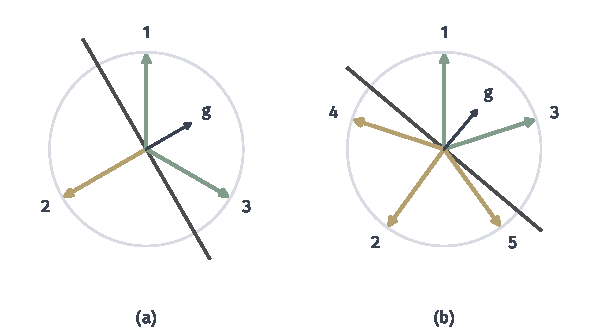
\includegraphics[width=100mm]{figures/05-optimization/06-constrained-optimization/matplotlib/cone-round-vectors/figure.pdf}
  \caption{随机超平面取整。深灰线是与随机方向$\bm{g}$垂直的直线，绿色向量对应$x_i=1$，黄色向量对应$x_i=-1$。(a)三角形问题的三个向量互成$120^\circ$。(b)五边形问题的五个向量，相邻编号之间夹角$144^\circ$。}
  \label{fig:cone-round-vectors}
\end{BookInlineFigure}

\paragraph{恢复可能破坏可行性}
取整会改变目标，也会破坏约束。设问题~\eqref{eq:cone-sign-problem}中$n=4$，再加上平衡约束$x_1+x_2+x_3+x_4=0$。把它平方后提升为$\langle\bm{1}\bm{1}^\top,\bm{X}\rangle=0$。矩阵
\[
 \bm{X}=\frac43\bm{I}-\frac13\bm{1}\bm{1}^\top
\]
对角元为$1$，非对角元为$-1/3$，特征值是$4/3,4/3,4/3,0$，且$\langle\bm{1}\bm{1}^\top,\bm{X}\rangle=4-12/3=0$，满足松弛的全部约束。

它对应四面体的四个顶点方向，这四个向量和为零，一个超平面不可能把它们全放在同一侧，取整结果只有两种：二比二（满足平衡约束）或一比三（$(\sum_ix_i)^2=4$，违反约束）。由式~\eqref{eq:cone-rounding-expectation}，
\[
 \mathbb{E}\Bigl[\bigl(\sum_ix_i\bigr)^2\Bigr]=4+12\cdot\frac2\pi\arcsin\Bigl(-\frac13\Bigr)\approx1.404.
\]
除以$4$，一比三的概率约为$0.351$。超过三分之一的取整结果是不可行的，必须修复或丢弃后重新检验。

\subsection{上下界检验}
\label{sec:cone-relax-bounds}

松弛算出来的数字到底保证了什么？这一小节把上界、下界和间隙分别交代清楚。

\paragraph{两个界}
一个经过原约束核对的点$\hat{\bm{x}}$给出上界$U=f(\hat{\bm{x}})$。一个松弛的对偶可行解$\bm{y}$给出下界$L$，对符号问题就是$L=\sum_iy_i$。合起来是一条链：
\begin{equation}
 L\leq p_{\mathrm{rel}}\leq f^\star\leq U.
 \label{eq:cone-bound-chain}
\end{equation}
报告时写出$U-L$。它同时包含松弛自身的间隙和求解的误差，是对$\hat{\bm{x}}$质量的一个可靠估计。

在三角形例子中，$U=-2$，$L=-3$，$U-L=1$。这里$\hat{\bm{x}}$其实已经最优，间隙全部来自松弛，继续迭代也不会缩小。间隙不为零，不代表候选解不好。

\paragraph{近似原始值不是下界}
常见的错误是把松弛问题的一个可行矩阵的目标值当作下界。式~\eqref{eq:cone-bound-chain}中排在$f^\star$左边的是$p_{\mathrm{rel}}$，而可行矩阵$\hat{\bm{X}}$的目标值满足的是
\[
 \langle\bm{W},\hat{\bm{X}}\rangle\geq p_{\mathrm{rel}},
\]
方向相反。它可以高于$f^\star$。

取三角形问题中对角元为$1$、非对角元为$-0.3$的矩阵，特征值是$0.4,1.3,1.3$，松弛可行，目标是$-1.8$。可$f^\star=-2<-1.8$。若把$-1.8$当作下界，就会错误地断言符号问题的最优值不低于$-1.8$，如图~\ref{fig:cone-bounds-line}所示。

\begin{BookInlineFigure}
  \centering
  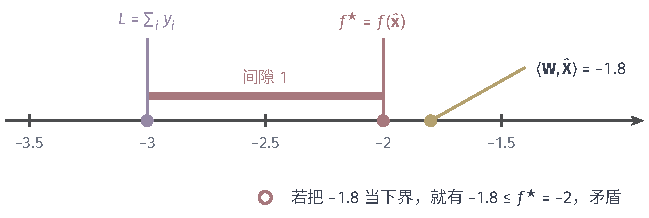
\includegraphics[width=110mm]{figures/05-optimization/06-constrained-optimization/tikz/cone-bounds-line/figure.pdf}
  \caption{三角形符号问题的各个数值。紫点是对偶可行解给出的下界$L=-3$，红点是最优值$f^\star=-2$，它也等于取整解的上界。黄点是松弛的一个未收敛可行矩阵的目标值$-1.8$，位于$f^\star$右侧，不能当作下界。红色粗线是报告的间隙。}
  \label{fig:cone-bounds-line}
\end{BookInlineFigure}

\paragraph{从近似对偶解得到有效下界}
数值求解器返回的$\bm{y}$往往只是近似可行，$\bm{W}-\operatorname{diag}(\bm{y})$可能有微小的负特征值，严格说来式~\eqref{eq:cone-bound-chain}不能用。幸好符号问题的对偶可行性很容易修复。

\begin{lemma}[修复对偶可行性]
\label{lem:cone-repair-dual}
对任意$\bm{y}\in\mathbb{R}^n$，记$\lambda$为矩阵$\bm{W}-\operatorname{diag}(\bm{y})$的最小特征值。则
\begin{equation}
 L(\bm{y})=\sum_{i=1}^ny_i+n\lambda
 \label{eq:cone-repaired-bound}
\end{equation}
是问题~\eqref{eq:cone-sign-relax}的最优值的下界，因而也是$f^\star$的下界。
\end{lemma}

\begin{proof}
令$\bm{y}'=\bm{y}+\lambda\bm{1}$。则
\[
 \bm{W}-\operatorname{diag}(\bm{y}')=\bm{W}-\operatorname{diag}(\bm{y})-\lambda\bm{I}\succeq\bm{0},
\]
因为最小特征值被平移到了零。所以$\bm{y}'$是问题~\eqref{eq:cone-sign-dual}的可行解，目标是$\sum_iy_i+n\lambda$。由弱对偶和定理~\ref{thm:cone-sdr-bound}得到结论。
\end{proof}

这个界对任何$\bm{y}$都成立，只要算得出最小特征值。例如在三角形问题中取不可行的$\bm{y}=(-1.1,-0.9,-1)$，最小特征值约为$-0.059$，修复后$L\approx-3.177$，仍是有效的下界。数值计算特征值本身有误差，严格的报告还要再减去一个反映舍入误差的小量。

图~\ref{fig:cone-bounds-iter}是一个$10$个变量的符号问题，权重是固定种子生成的$\pm1$。枚举全部符号组合得到$f^\star=-46$。求解松弛时，绿线是原始可行矩阵的目标值，紫线是由式~\eqref{eq:cone-repaired-bound}修复的下界。

\begin{BookInlineFigure}
  \centering
  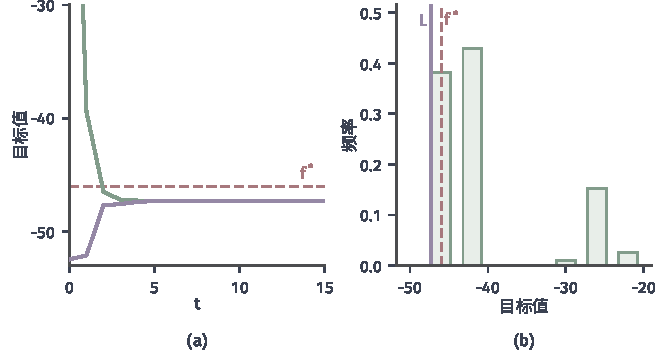
\includegraphics[width=112mm]{figures/05-optimization/06-constrained-optimization/matplotlib/cone-bounds-iter/figure.pdf}
  \caption{$n=10$的符号问题（$\bm{W}$的非对角元为随机$\pm1$，种子$7$）。(a)松弛的求解过程：绿线是可行矩阵的目标值，紫线是修复后的对偶下界，红色虚线是枚举得到的$f^\star=-46$。前两步绿线高于$f^\star$，不是$f^\star$的下界；收敛后二者相遇在$L\approx-47.28$。(b)从最终矩阵取整$2000$次得到的目标值分布，紫线是$L$，红色虚线是$f^\star$。}
  \label{fig:cone-bounds-iter}
\end{BookInlineFigure}

绿线在开始两步高于$f^\star$，把它当下界会得到错误的结论。收敛后两条线都停在$-47.28$附近，这就是$p_{\mathrm{rel}}$，它比$f^\star$低约$1.28$。这段距离是放松秩约束的代价，再多的迭代也消除不了。

图的(b)部分取整$2000$次。约$38\%$的试验得到$-46$，也就是真实最优值；其余的目标更差，最差到$-22$。所以取整要重复多次，取其中最好的可行点作为上界。这里$U=-46$，$U-L\approx1.28$，已经足以说明候选解很接近最优。

表~\ref{tab:cone-reported-quantities}整理了各个量的含义和要做的核对。

\begin{BookInlineTable}
  \centering
  \begin{tabular}{lll}
    \toprule
    量 & 保证 & 需要核对\\
    \midrule
    $f(\hat{\bm{x}})$ & $f^\star$的上界 & $\hat{\bm{x}}$满足原约束\\
    $\sum_iy_i$ & $f^\star$的下界 & $\bm{y}$对偶可行\\
    $\langle\bm{W},\hat{\bm{X}}\rangle$ & 收敛时接近$p_{\mathrm{rel}}$ & 不是$f^\star$的界\\
    $U-L$ & 候选解的最优性间隙 & 上下两界都已核对\\
    \bottomrule
  \end{tabular}
  \caption{半正定松弛的结果中各个量的含义。}
  \label{tab:cone-reported-quantities}
\end{BookInlineTable}

\section{模型与求解方法}
\label{sec:cone-methods}

同一个问题可以有多种写法。于是要问：写法不同时，变量规模、存储和运算量分别差多少，应该按什么选择？

\paragraph{同一个问题的三种写法}
预算问题已经写过三遍：原变量的二次规划、式~\eqref{eq:cone-qp-socp}的二阶锥形式，以及用式~\eqref{eq:cone-schur-quadratic}得到的线性矩阵不等式。三者等价，解都是$(3/2,1/2)$，规模却不同。表~\ref{tab:cone-three-forms}列出例子（$n=2$，$k=3$）和一般情形。

\begin{BookInlineTable}
  \centering
  \begin{tabular}{llll}
    \toprule
    & 二次规划 & 二阶锥形式 & 线性矩阵不等式\\
    \midrule
    变量 & $2$（一般$n$） & $3$（$n+1$） & $3$（$n+1$）\\
    非线性结构 & $\bm{Q}$，$2\times2$ & $5$维锥（$k+2$） & $4\times4$（$k+1$阶）\\
    矩阵独立元素 & $3$ & 无 & $10$\\
    恢复原变量 & 直接 & 丢弃$t$ & 丢弃$t$\\
    \bottomrule
  \end{tabular}
  \caption{预算问题的三种等价写法。括号内是一般规模：$n$个变量，$\bm{F}\in\mathbb{R}^{k\times n}$。线性约束三者相同，未列出。}
  \label{tab:cone-three-forms}
\end{BookInlineTable}

\paragraph{模型的包含关系}
图~\ref{fig:cone-hierarchy}把前面的改写连成一条链。线性规划是$\bm{Q}=\bm{0}$的二次规划；凸二次规划由式~\eqref{eq:cone-qp-socp}写成二阶锥规划；二阶锥规划由式~\eqref{eq:cone-soc-as-lmi}写成半正定规划。

\begin{BookInlineFigure}
  \centering
  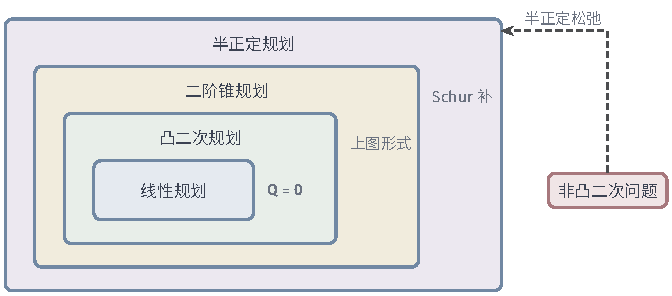
\includegraphics[width=112mm]{figures/05-optimization/06-constrained-optimization/tikz/cone-hierarchy/figure.pdf}
  \caption{模型的包含关系。边框旁标注内层写成外层所用的改写。非凸二次问题不在这条链上，它只能经半正定松弛（虚线）得到下界。}
  \label{fig:cone-hierarchy}
\end{BookInlineFigure}

这条链说的是表达能力，不是推荐的求解路线。外层的模型能表达内层的问题，但内层的结构在外层看不见了。一个$k+2$维的二阶锥写成线性矩阵不等式后，要用$(k+1)\times(k+1)$的矩阵，存储从$O(k)$变成$O(k^2)$。

内点法每步解一个线性方程，按稠密数据粗略估计：$n$个变量的二次规划，每步约$O(n^3)$次运算；变量为$n$、矩阵阶为$k$的线性矩阵不等式，组装牛顿方程的系数矩阵就要$O(nk^3+n^2k^2)$次，分解再要$O(n^3)$次\scite{math-boyd2004convex}。所以能用内层模型时就不要往外走。

\paragraph{松弛的规模}
半正定松弛的规模增长更快。问题~\eqref{eq:cone-sign-relax}把$n$个变量换成$n\times n$的矩阵。$n=1000$时，矩阵存储$10^6$个数，独立的非对角元有$n(n-1)/2=499500$个，一次特征分解约$10^9$次运算。此外还要重复取整和验证。松弛的结果换来的是一个下界，这个下界是否值得这样的代价，要看问题规模和对全局证据的需要。

\paragraph{各类方法的去向}
后面几章给出具体的算法，这里只说明各自处理什么情形。第~\ref{chap:sequential-quadratic-programming}章把二次规划当作子问题反复求解。第~\ref{chap:nonlinear-interior-point}章把第~\ref{chap:lp-interior-point}章的内点法推广到一般光滑约束和锥约束。

若可行集的投影便宜，或约束可以拆成几块分别处理，第~\ref{chap:feasible-iterations}章和第~\ref{chap:penalty-multiplier-methods}章的方法每步代价低得多，适合只需中等精度的大规模问题。

投影到半正定锥就是一个例子：作谱分解，把负特征值截成零。例如$\begin{bmatrix}1&2\\2&1\end{bmatrix}$的特征值是$3$和$-1$，特征向量是$(1,1)/\sqrt2$和$(1,-1)/\sqrt2$。截断负特征值后得到
\[
 3\cdot\frac12\begin{bmatrix}1&1\\1&1\end{bmatrix}=\frac32\begin{bmatrix}1&1\\1&1\end{bmatrix}.
\]
一次投影需要一次完整的特征分解，代价约$O(n^3)$，这决定了这类方法能处理的矩阵阶数。

\paragraph{选择的依据}
选择模型时可以按下面的顺序问。

\begin{enumerate}
 \item 问题是否凸？不凸的话，改写不会改变这一点，只能走局部方法或松弛。
 \item 能否停留在最内层的模型？线性约束的凸二次问题就用二次规划，不要因为通用求解器方便而升级。
 \item 数据有什么结构？稀疏、低秩或只能做矩阵向量积，决定是否可以分解，也决定内点法和一阶方法哪个更合算。
 \item 需要什么样的结论？只要一个好的解，局部方法足够；需要全局证据，就要付出松弛和对偶验证的代价。
\end{enumerate}

无论走哪条路，得到结果后都要分别核对，如图~\ref{fig:cone-workflow}所示。等价改写的解丢弃辅助变量后可以直接用，松弛的解则要先恢复再验证。

\begin{BookInlineFigure}
  \centering
  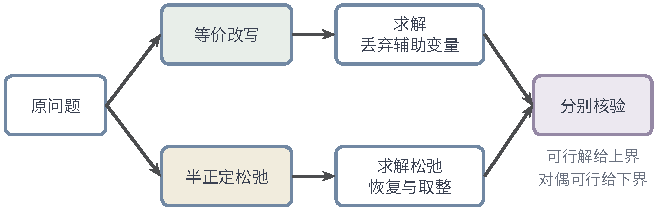
\includegraphics[width=110mm]{figures/05-optimization/06-constrained-optimization/tikz/cone-workflow/figure.pdf}
  \caption{从原问题到可靠结论的两条路径。等价改写（绿）保持最优解，求解后丢弃辅助变量。半正定松弛（黄）扩大可行集，求解后要恢复原变量。两条路径最后都要分别核验：可行解给出上界，对偶可行解给出下界。}
  \label{fig:cone-workflow}
\end{BookInlineFigure}

\section{本章小结}
\label{sec:cone-summary}

章首的三件事现在有了各自的归属。带预算的最小二乘是凸二次规划，距离上限的交集是二阶锥规划，相关系数的可行范围由半正定约束决定。把问题写成这些标准形式，是为了把目标的曲率、可行集的形状和可检验的对偶界摆到明面上。

二次规划要看的是$\bm{Q}$在可行差方向上的曲率，而不是全空间。这一曲率决定凸性和唯一性；凸时KKT条件是全局证书，非凸时KKT点可以是局部极小点或鞍点，证书不再成立。等式约束的情形化为线性方程，方程可逆只保证驻点唯一，极小性还要看约化Hessian。

锥规划把非负约束换成闭凸锥，乘子换成对偶锥的元素。弱对偶无条件成立，给出的下界可以直接验证；强对偶和最优解的达到则需要严格可行性等条件，线性规划的结论不能原样搬到半正定规划。

表~\ref{tab:cone-summary}比较后半章的两种操作。

\begin{BookInlineTable}
  \centering
  \begin{tabular}{lll}
    \toprule
    & 等价改写 & 半正定松弛\\
    \midrule
    可行集 & 投影后与原集合相同 & 严格扩大（一般情形）\\
    最优值 & 相等 & 不超过原最优值\\
    恢复原变量 & 丢弃辅助变量 & 秩一时直接读出，否则取整\\
    所需核对 & 改写的两个方向 & 可行性、对偶可行性、间隙\\
    典型工具 & 上图形式、Schur补 & 提升、删秩、随机取整\\
    \bottomrule
  \end{tabular}
  \caption{等价改写与半正定松弛的对比。}
  \label{tab:cone-summary}
\end{BookInlineTable}

算法返回的矩阵、原问题的可行解和最优性证书是三样不同的东西，需要分别检查。松弛最优矩阵不一定对应可行点，近似的原始值不是下界，只有经原约束核对的点给出上界，只有对偶可行的解给出下界，两者之差才是可以报告的结论。

